\documentclass[a4paper,12pt,twoside]{memoir}

% Castellano
\usepackage[spanish,es-tabla]{babel}
\selectlanguage{spanish}
\usepackage[utf8]{inputenc}
\usepackage[T1]{fontenc}
\usepackage{lmodern} % Scalable font
\usepackage{microtype}
\usepackage{placeins}
%Packs Elsa
\usepackage{algpseudocode}
\usepackage{algorithm}
\usepackage{amsmath}


\RequirePackage{booktabs}
\RequirePackage[table]{xcolor}
\RequirePackage{xtab}
\RequirePackage{multirow}

% Links
\PassOptionsToPackage{hyphens}{url}\usepackage[colorlinks]{hyperref}
\hypersetup{
	allcolors = {red}
}

% Cambiar el nombre del título de la lista de algoritmos
\addto\captionsspanish{\renewcommand{\listalgorithmname}{Índice de Algoritmos}}

% Ecuaciones
\usepackage{amsmath}

% Rutas de fichero / paquete
\newcommand{\ruta}[1]{{\sffamily #1}}

% Párrafos
\nonzeroparskip

% Huérfanas y viudas
\widowpenalty100000
\clubpenalty100000

% Imagenes
\usepackage{graphicx}
\newcommand{\imagen}[2]{
	\begin{figure}[!h]
		\centering
		\includegraphics[width=0.9\textwidth]{#1}
		\caption{#2}\label{fig:#1}
	\end{figure}
	\FloatBarrier
}

\newcommand{\imagenflotante}[2]{
	\begin{figure}%[!h]
		\centering
		\includegraphics[width=0.9\textwidth]{#1}
		\caption{#2}\label{fig:#1}
	\end{figure}
}



% El comando \figura nos permite insertar figuras comodamente, y utilizando
% siempre el mismo formato. Los parametros son:
% 1 -> Porcentaje del ancho de página que ocupará la figura (de 0 a 1)
% 2 --> Fichero de la imagen
% 3 --> Texto a pie de imagen
% 4 --> Etiqueta (label) para referencias
% 5 --> Opciones que queramos pasarle al \includegraphics
% 6 --> Opciones de posicionamiento a pasarle a \begin{figure}
\newcommand{\figuraConPosicion}[6]{%
  \setlength{\anchoFloat}{#1\textwidth}%
  \addtolength{\anchoFloat}{-4\fboxsep}%
  \setlength{\anchoFigura}{\anchoFloat}%
  \begin{figure}[#6]
    \begin{center}%
      \Ovalbox{%
        \begin{minipage}{\anchoFloat}%
          \begin{center}%
            \includegraphics[width=\anchoFigura,#5]{#2}%
            \caption{#3}%
            \label{#4}%
          \end{center}%
        \end{minipage}
      }%
    \end{center}%
  \end{figure}%
}

%
% Comando para incluir imágenes en formato apaisado (sin marco).
\newcommand{\figuraApaisadaSinMarco}[5]{%
  \begin{figure}%
    \begin{center}%
    \includegraphics[angle=90,height=#1\textheight,#5]{#2}%
    \caption{#3}%
    \label{#4}%
    \end{center}%
  \end{figure}%
}
% Para las tablas
\newcommand{\otoprule}{\midrule [\heavyrulewidth]}
%
% Nuevo comando para tablas pequeñas (menos de una página).
\newcommand{\tablaSmall}[5]{%
 \begin{table}
  \begin{center}
   \rowcolors {2}{gray!35}{}
   \begin{tabular}{#2}
    \toprule
    #4
    \otoprule
    #5
    \bottomrule
   \end{tabular}
   \caption{#1}
   \label{tabla:#3}
  \end{center}
 \end{table}
}

%
% Nuevo comando para tablas pequeñas (menos de una página).
\newcommand{\tablaSmallSinColores}[5]{%
 \begin{table}[H]
  \begin{center}
   \begin{tabular}{#2}
    \toprule
    #4
    \otoprule
    #5
    \bottomrule
   \end{tabular}
   \caption{#1}
   \label{tabla:#3}
  \end{center}
 \end{table}
}

\newcommand{\tablaApaisadaSmall}[5]{%
\begin{landscape}
  \begin{table}
   \begin{center}
    \rowcolors {2}{gray!35}{}
    \begin{tabular}{#2}
     \toprule
     #4
     \otoprule
     #5
     \bottomrule
    \end{tabular}
    \caption{#1}
    \label{tabla:#3}
   \end{center}
  \end{table}
\end{landscape}
}

%
% Nuevo comando para tablas grandes con cabecera y filas alternas coloreadas en gris.
\newcommand{\tabla}[6]{%
  \begin{center}
    \tablefirsthead{
      \toprule
      #5
      \otoprule
    }
    \tablehead{
      \multicolumn{#3}{l}{\small\sl continúa desde la página anterior}\\
      \toprule
      #5
      \otoprule
    }
    \tabletail{
      \hline
      \multicolumn{#3}{r}{\small\sl continúa en la página siguiente}\\
    }
    \tablelasttail{
      \hline
    }
    \bottomcaption{#1}
    \rowcolors {2}{gray!35}{}
    \begin{xtabular}{#2}
      #6
      \bottomrule
    \end{xtabular}
    \label{tabla:#4}
  \end{center}
}

%
% Nuevo comando para tablas grandes con cabecera.
\newcommand{\tablaSinColores}[6]{%
  \begin{center}
    \tablefirsthead{
      \toprule
      #5
      \otoprule
    }
    \tablehead{
      \multicolumn{#3}{l}{\small\sl continúa desde la página anterior}\\
      \toprule
      #5
      \otoprule
    }
    \tabletail{
      \hline
      \multicolumn{#3}{r}{\small\sl continúa en la página siguiente}\\
    }
    \tablelasttail{
      \hline
    }
    \bottomcaption{#1}
    \begin{xtabular}{#2}
      #6
      \bottomrule
    \end{xtabular}
    \label{tabla:#4}
  \end{center}
}

%
% Nuevo comando para tablas grandes sin cabecera.
\newcommand{\tablaSinCabecera}[5]{%
  \begin{center}
    \tablefirsthead{
      \toprule
    }
    \tablehead{
      \multicolumn{#3}{l}{\small\sl continúa desde la página anterior}\\
      \hline
    }
    \tabletail{
      \hline
      \multicolumn{#3}{r}{\small\sl continúa en la página siguiente}\\
    }
    \tablelasttail{
      \hline
    }
    \bottomcaption{#1}
  \begin{xtabular}{#2}
    #5
   \bottomrule
  \end{xtabular}
  \label{tabla:#4}
  \end{center}
}



\definecolor{cgoLight}{HTML}{EEEEEE}
\definecolor{cgoExtralight}{HTML}{FFFFFF}

%
% Nuevo comando para tablas grandes sin cabecera.
\newcommand{\tablaSinCabeceraConBandas}[5]{%
  \begin{center}
    \tablefirsthead{
      \toprule
    }
    \tablehead{
      \multicolumn{#3}{l}{\small\sl continúa desde la página anterior}\\
      \hline
    }
    \tabletail{
      \hline
      \multicolumn{#3}{r}{\small\sl continúa en la página siguiente}\\
    }
    \tablelasttail{
      \hline
    }
    \bottomcaption{#1}
    \rowcolors[]{1}{cgoExtralight}{cgoLight}

  \begin{xtabular}{#2}
    #5
   \bottomrule
  \end{xtabular}
  \label{tabla:#4}
  \end{center}
}



\graphicspath{ {./img/} }

% Capítulos
\chapterstyle{bianchi}
\newcommand{\capitulo}[2]{
	\setcounter{chapter}{#1}
	\setcounter{section}{0}
	\setcounter{figure}{0}
	\setcounter{table}{0}
	\chapter*{#2}
	\addcontentsline{toc}{chapter}{#2}
	\markboth{#2}{#2}
}

% Apéndices
\renewcommand{\appendixname}{Apéndice}
\renewcommand*\cftappendixname{\appendixname}

\newcommand{\apendice}[1]{
	%\renewcommand{\thechapter}{A}
	\chapter{#1}
}

\renewcommand*\cftappendixname{\appendixname\ }

% Formato de portada
\makeatletter
\usepackage{xcolor}
\newcommand{\tutor}[1]{\def\@tutor{#1}}
\newcommand{\course}[1]{\def\@course{#1}}
\definecolor{cpardoBox}{HTML}{E6E6FF}
\def\maketitle{
  \null
  \thispagestyle{empty}
  % Cabecera ----------------
\noindent
\includegraphics[width=\textwidth]{cabecera}\vspace{1cm}%
  \vfill
  % Título proyecto y escudo informática ----------------
  \colorbox{cpardoBox}{%
    \begin{minipage}{.8\textwidth}
      \vspace{.5cm}\Large
      \begin{center}
      \textbf{TFG del Grado en Ingeniería Informática}\vspace{.6cm}\\
      \textbf{\LARGE\@title{}}
      \end{center}
      \vspace{.2cm}
    \end{minipage}

  }%
  \hfill\begin{minipage}{.20\textwidth}
    
\includegraphics[width=\textwidth]{escudoInfor}
  \end{minipage}
  \vfill
  % Datos de alumno, curso y tutores ------------------
  \begin{center}%
  {%
    \noindent\LARGE
    Presentado por \@author{}\\ 
    en Universidad de Burgos --- \@date{}\\
    Tutor: \@tutor{}\\
  }%
  \end{center}%
  \null
  \cleardoublepage
  }
\makeatother

\newcommand{\nombre}{Elsa Tolín Carrasco} %%% cambio de comando

% Datos de portada
\title{Algoritmos y mazmorras}
\author{\nombre}
\tutor{José Manuel Galán Ordax y Jesús Alonso Abad}

\date{\today}


\begin{document}

\maketitle


\newpage\null\thispagestyle{empty}\newpage


%%%%%%%%%%%%%%%%%%%%%%%%%%%%%%%%%%%%%%%%%%%%%%%%%%%%%%%%%%%%%%%%%%%%%%%%%%%%%%%%%%%%%%%%
% \thispagestyle{empty}


% \noindent
\includegraphics[width=\textwidth]{cabecera}\vspace{1cm}

% \noindent D. Jose Manuel Galan Ordax, profesor del departamento de nombre departamento, área de nombre área.

% \noindent Expone:

% \noindent Que el alumno D. \nombre, con DNI dni, ha realizado el Trabajo final de Grado en Ingeniería Informática titulado título de TFG. 

% \noindent Y que dicho trabajo ha sido realizado por el alumno bajo la dirección del que suscribe, en virtud de lo cual se autoriza su presentación y defensa.

% \begin{center} %\large
% En Burgos, {\large \today}
% \end{center}

% \vfill\vfill\vfill

% % Author and supervisor
% \begin{minipage}{0.45\textwidth}
% \begin{flushleft} %\large
% Vº. Bº. del Tutor:\\[2cm]
% D. nombre tutor
% \end{flushleft}
% \end{minipage}
% \hfill
% \begin{minipage}{0.45\textwidth}
% \begin{flushleft} %\large
% Vº. Bº. del co-tutor:\\[2cm]
% D. nombre co-tutor
% \end{flushleft}
% \end{minipage}
% \hfill

% \vfill

% para casos con solo un tutor comentar lo anterior
% y descomentar lo siguiente
%Vº. Bº. del Tutor:\\[2cm]
%D. nombre tutor





\frontmatter

% Abstract en castellano
\renewcommand*\abstractname{Resumen}
\begin{abstract}
La generación procedimental es una técnica de generación de contenido que hace uso de algoritmos para obtener mapas, texturas, niveles, historias...
En este proyecto se va a realizar un videojuego que utilice esta técnica y se van a explorar varios algoritmos para poder ver sus resultados y tiempos de ejecución.
\end{abstract}

\renewcommand*\abstractname{Descriptores}
\begin{abstract}
Generación procedimental, API, Docker, DevContainer, Unity, Base de datos NoSQL \ldots
\end{abstract}

\clearpage

% Abstract en inglés
\renewcommand*\abstractname{Abstract}
\begin{abstract}
Procedural generation is a content generation technique which uses algorithms to obtain maps, textures, levels, stories...
To make use of this technique, a videogame will be developed which uses several procedural generation algorithms, together with an exploration of the results and execution time.
\end{abstract}

\renewcommand*\abstractname{Keywords}
\begin{abstract}
Procedural generation, API, Docker, DevContainer, Unity, NoSQL database \ldots
\end{abstract}

\clearpage

% Indices
\tableofcontents

\clearpage

\listoffigures

\clearpage

\listoftables

\listofalgorithms

\clearpage

\mainmatter
\capitulo{1}{Introducción}

La generación procedimental, es la técnica que a través de algoritmos, permite crear contenido para videojuegos de forma autónoma o de la mano de un diseñador. 
Usar esta técnica permite optimizar o crear videojuegos que tengan la posibilidad de crear nuevos escenarios completamente nuevos para cada jugador.

Esta técnica forma parte de algunos videojuegos que llevan publicados más de tres décadas, y a día de hoy es una técnica muy popular que es utilizada en juegos muy reconocidos. Uno de sus usos más populares y reconocidos es para la creación de mapas para videojuegos o incluso juegos de mesa. 

Es por ello que para este trabajo de fin de grado, se van a explorar distintos algoritmos para poder probar esta técnica, de forma que se obtengan mapas navegables como lo serían en un videojuego. Estos mapas van a tener la forma de un laberinto y van a ser generados en un servidor, replicando la arquitectura que se tendría en un estudio de videojuegos real.



\capitulo{2}{Objetivos del proyecto}
Este proyecto tiene como objetivo principal la creación de un videojuego destinado a la generación automática de laberintos navegables por el usuario a partir de algoritmos de generación procedimental en un motor de videojuegos. Los objetivos para llevar a cabo el proyecto son los siguientes:

\begin{enumerate}
    \item Obtener laberintos que sean navegables.
    \item Utilizar varios algoritmos de generación procedimental para generar dichos laberintos.
    \item Usar la arquitectura cliente-servidor para poder almacenar datos del videojuego.
    \item Utilizar el protocolo HTTP para que el servidor se comunique con Unity.
    \item Calcular los tiempos de ejecución de estos algoritmos y compararlos.
    \item Generar una imagen del contenido con Docker para que se pueda alojar fácilmente en un servidor externo.
\end{enumerate}
\capitulo{3}{Conceptos teóricos}

En la presente sección se describen los principales conceptos teóricos con los que se ha trabajado a lo largo del proyecto. Estos fundamentos teóricos permitirán una mejor comprensión del producto final.

\section{Generación procedimental}
La generación procedimental, es la generación algorítmica de contenido de forma automática. Se podría decir en otras palabras que se refiere a un software que puede crear contenido de forma independiente sin necesidad de una persona que lo diseñe~\cite{proceduralgenbooknoor}.

Este concepto, si lo aplicamos a un videojuego, implica generar contenido de forma ilimitada, sin necesidad de un diseñador. El contenido que se puede generar abarca desde texturas, mapas, niveles, historias, música, armas, personajes, etc. Surgió para reducir costes y tiempo de desarrollo y para proporcionar una experiencia de juego única.

\subsection{Origen y ejemplos}
Los primeras aplicaciones de la generación procedimental en videojuegos se remonta a las primeras décadas del desarrollo de software de entretenimiento; había falta de recursos de almacenamiento y se necesitaban métodos eficientes para poder crear grandes volúmenes de contenido. Uno de los primeros juegos en usar generación procedimental es \textbf{<<Rogue>>}(1980). En este juego se usaba la generación procedimental para generar niveles de mazmorra de forma aleatoria en cada partida, así se podía obtener una experiencia completamente distinta en cada sesión, como se muestra en la figura \ref{fig:CaputraRogue}~\cite{proceduralgenbooknoor}.
\begin{figure}[h!]  
    \centering  
    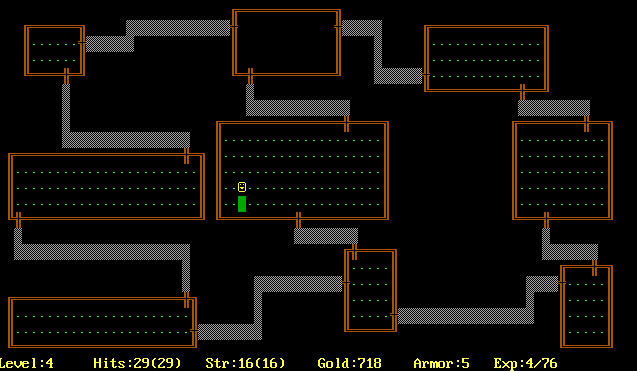
\includegraphics[width=\textwidth]{img/Rogue_Captura.PNG}  
    \caption{Captura del juego <<Rogue>>. Extraída de \url{https://es.wikipedia.org/wiki/Rogue.}}  
    \label{fig:CaputraRogue}
\end{figure}

\textbf{<<Minecraft>>} es otro ejemplo de juego que utiliza generación procedimental para los mapas. En el caso de este juego los mundos se generan de forma procedimental usando la función matemática \textbf{<<Ruido Perlin>>}\footnote{El <<Ruido Perlin>> hace uso de una interpolación entre un gran número de gradientes precalculados, construyen de esta forma un valor que varía, similar al ruido blanco y se utiliza para generar imágenes.\cite{wikipediaPerlin}} modificado, de esta forma crea terrenos, biomas y cuevas únicas cada vez que se inicia el juego. Esto permite crear un mundo muy extenso y variado sin la necesidad de diseñarlos manualmente~\cite{proceduralgenbooknoor}.

Pero el mejor ejemplo de juego procedimental es \textbf{<<No Man's Sky>>}. Este juego consigue crear mundos y universos de forma procedimental. A través de multitud de algoritmos complejos consigue crear planetas enteros, incluyendo la flora, fauna y paisajes, como se muestra en la figura \ref{fig:CaputraNoMansSky}. Este juego proporciona una experiencia de exploración infinita, esta capacidad de generación procedimental ha permitido a este juego crear un entorno expansivo que no se podría crear manualmente~\cite{proceduralgenbooknoor}.
\begin{figure}[h!]  
    \centering  
    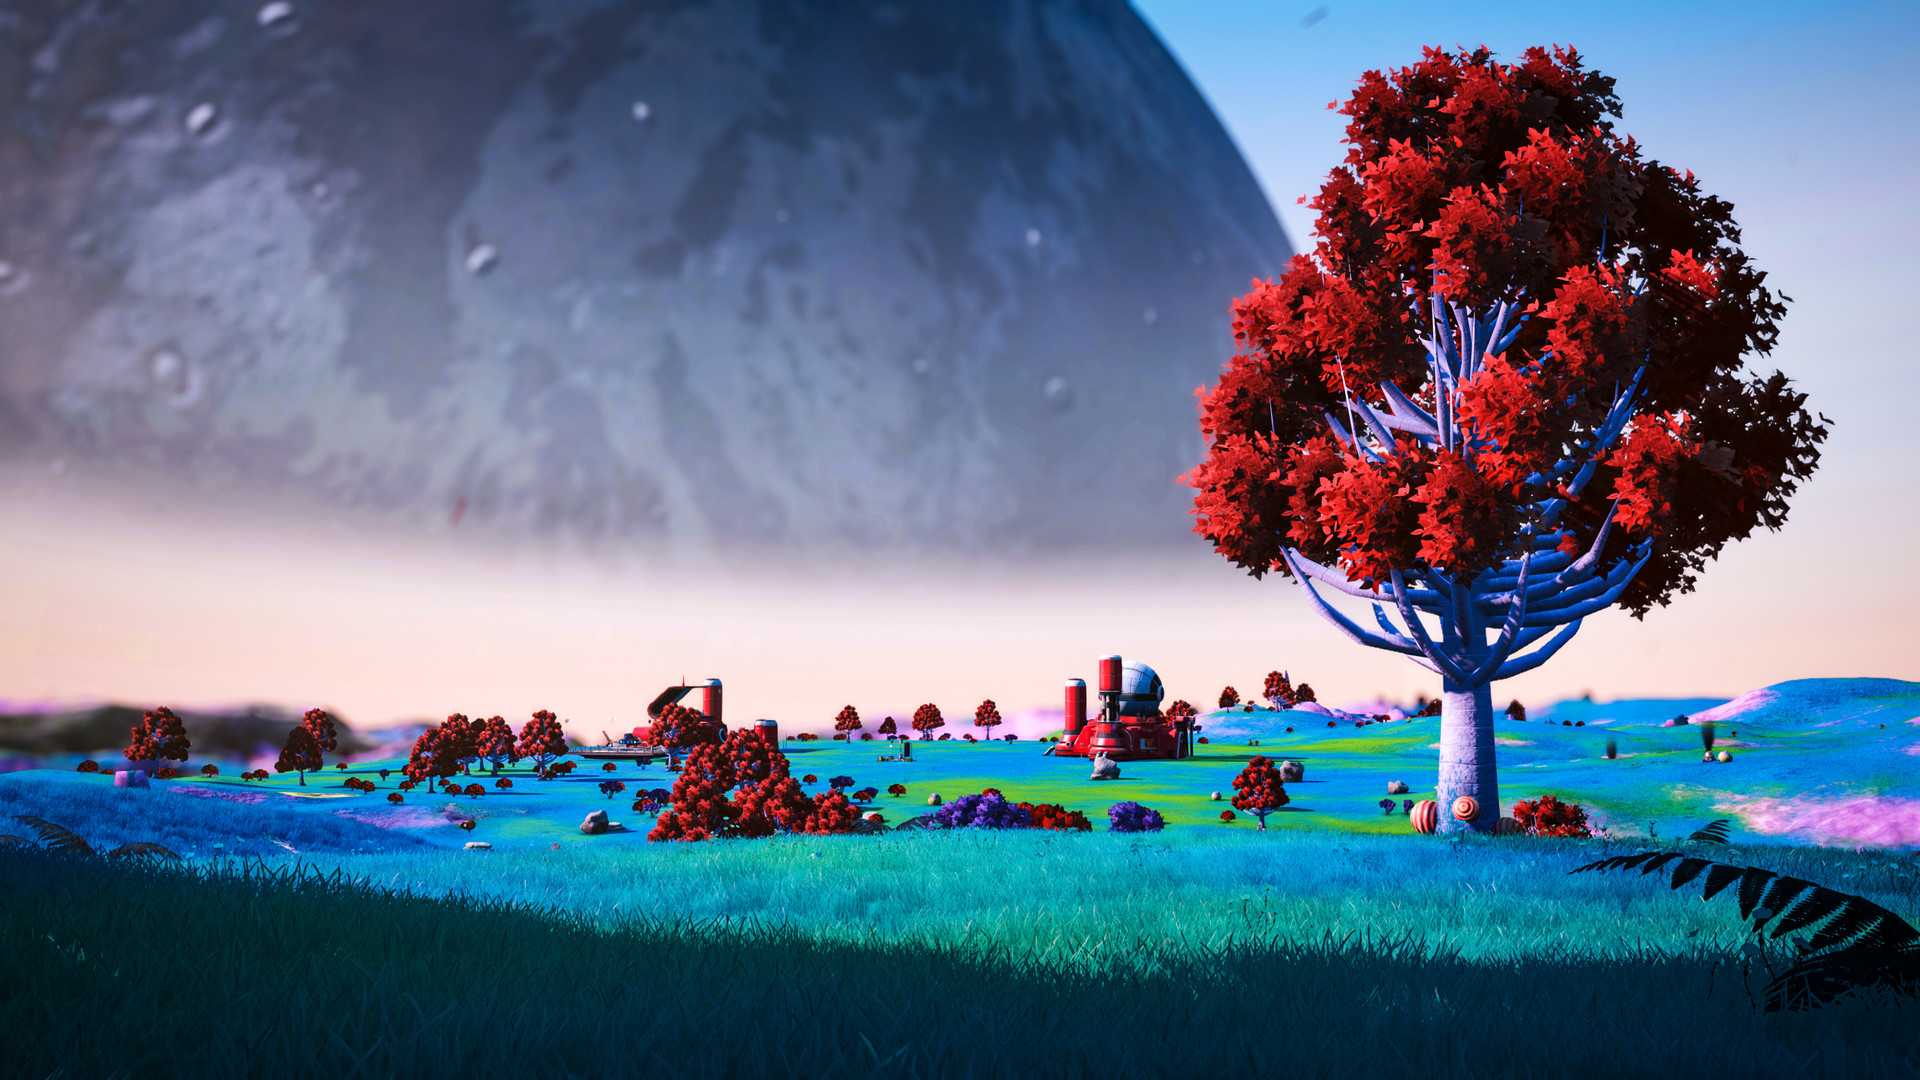
\includegraphics[width=\textwidth]{img/NoMansSkyScreenShot.jpg}  
    \caption{Captura del juego <<No Man's Sky>>. Extraída de \url{https://www.artstation.com/artwork/gEZ9P?album_id=660885}}  
    \label{fig:CaputraNoMansSky}
\end{figure}

\section{Algoritmos}
\subsection{Algoritmo de Prim}
El algoritmo de Prim, se ha usado tradicionalmente para encontrar el árbol de expansión mínima en un grafo, esto se puede adaptar para generar laberintos. Para adaptarlo, se seleccionan caminos aleatoriamente desde una celda inicial, y se va a expandir de forma que se mantenga la conectividad del laberinto sin crear ciclos, creando un camino único entre cualquier par de celdas~\cite{MazeGenAnalysis}.

Para poder generar el laberinto, en este caso el algoritmo se ha adaptado usando un enfoque que expande caminos desde una celda inicial y agrega aleatoriamente celdas vecinas a la estructura del laberinto. Así se puede asegurar de que se mantienen caminos únicos entre celdas, no se crean ciclos innecesarios y se genera un laberinto completamente conectado sin caminos redundantes. Funciona de una forma similar a cómo tradicionalmente se selecciona el arista más barato para expandir el árbol en un grafo.


\begin{algorithm}
\caption{Algoritmo DungeonPrim}
\begin{algorithmic}[1]
\Require Ancho $w$, alto $h$, semilla $s$ (opcional)
\Ensure Generar un laberinto usando el algoritmo de Prim

\State Inicializar la cuadrícula de mazmorra con tamaño $w \times h$
\If{$s \neq \text{None}$}
    \State Establecer semilla aleatoria $s$
\EndIf

\State Elegir una celda inicial $start$ aleatoria
\State Cambiar estado de $start$ a \texttt{PATH}
\State Agregar posición de $start$ a $steps$
\State $frontier\_set \gets$ vecinos de $start$ a distancia 2

\While{$frontier\_set$ no esté vacío}
    \State Elegir una celda $frontier\_cell$ aleatoria de $frontier\_set$
    \State Eliminar $frontier\_cell$ de $frontier\_set$

    \State \small{$frontier\_neighs \gets$ vecinos de $frontier\_cell$ a distancia 2 que sean \texttt{PATH}}
    \State Elegir una celda $connect\_cell$ aleatoria de $frontier\_neighs$

    \State Cambiar estado de $frontier\_cell$ a \texttt{PATH}
    \State Agregar posición de $frontier\_cell$ a $steps$

    \State Cambiar estado de la celda entre $frontier\_cell$ y $connect\_cell$ a \texttt{PATH}

    \State $new\_neighbors \gets$ vecinos de $frontier\_cell$ a distancia 2 que sean \texttt{WALL}
    \State Agregar $new\_neighbors$ a $frontier\_set$
\EndWhile

\State Definir $exit$ como la última celda conectada

\end{algorithmic}
\end{algorithm}


\subsection{Depth First Search-DFS}
El algoritmo de búsqueda de profundidad (DFS) es un algoritmo que se utiliza en la teoría de grafos y en árboles, para buscar caminos y soluciones en profundidad antes de retroceder. Este algoritmo se puede adaptar para crear laberintos con múltiples caminos y conexiones, asegurando que va a haber una solución de navegación sin realizar ciclos innecesarios~\cite{MazeGenAnalysis}.

En este caso, desde la celda inicial, el algoritmo explora en profundidad antes de retroceder y probar otro camino, y se crea un camino marcando las celdas como parte del laberinto mientras elimina los muros entre celdas adyacentes.
Los vecinos se barajan aleatoriamente para asegurar que el laberinto generado tenga una estructura impredecible y no se vean patrones evidentes.

\begin{algorithm}
\caption{Algoritmo DungeonDFS}
\begin{algorithmic}[1]
\Require Ancho $w$, alto $h$, semilla $s$ (opcional)
\Ensure Generar laberintos usando búsqueda en profundidad (DFS)

\State Inicializar la cuadrícula de mazmorra con tamaño $w \times h$
\If{$s \neq \text{None}$}
    \State Establecer semilla aleatoria $s$
\EndIf

\State Elegir una celda inicial $start$ aleatoria
\State Llamar a \texttt{hacer\_caminos($start$)}

\Procedure{hacer\_caminos}{cell, from\_cell}
    \State Cambiar estado de $cell$ a \texttt{PATH}
    \If{from\_cell $\neq$ None}
        \State Cambiar estado de la celda entre $cell$ y $from\_cell$ a \texttt{PATH}
        \State Agregar posición de la celda intermedia a $steps$
    \EndIf

    \State Obtener vecinos $random\_neighs$ de $cell$ a distancia 2
    \State Mezclar aleatoriamente $random\_neighs$

    \For{neigh en $random\_neighs$}
        \State Definir $exit$ como $neigh$
        \If{$neigh.state = \text{PATH}$}
            \State \textbf{continuar}
        \EndIf
        \State Llamar a \texttt{hacer\_caminos($neigh$, $cell$)}
    \EndFor
\EndProcedure

\Function{obtener\_celda\_entre}{origin, target}
    \State $(row\_origin, col\_origin) \gets origin.\text{get\_position}()$
    \State $(row\_target, col\_target) \gets target.\text{get\_position}()$

    \If{$row\_origin = row\_target$}
        \State \Return grid[$row\_origin$][max($col\_origin$, $col\_target$) - 1]
    \Else
        \State \Return grid[max($row\_origin$, $row\_target$) - 1][$col\_origin$]
    \EndIf
\EndFunction

\end{algorithmic}
\end{algorithm}



\subsection{Autómata celular}
Un autómata celular es un modelo matemático que se compone por una cuadrícula de celdas, cada una de las celdas puede estar en un estado finito, uno o cero. Esta cuadrícula va a evolucionar a lo largo de una serie de iteraciones, en el que el estado de cada celda en la siguiente iteración se determina en función de su estado actual y las celdas vecinas según unas reglas locales y uniformes. Para que pueda comenzar, se necesita proveer un estado inicial al algoritmo~\cite{cellularAutomata}.

Es similar a <<El juego de la vida>> de Conway, en el que las celdas van evolucionando a lo largo del tiempo en función de una serie de reglas y se va cambiando su estado de viva a muerta~\cite{wikipediaMazeGeneration}.


En este caso se ha adaptado de forma que en cada iteración se crea una nueva cuadrícula basada en la cuadrícula actual. Para comenzar, se le provee de unas celdas en estado de camino al algoritmo. Tras ese crea una copia de la cuadrícula actual para no modificar la cuadrícula original durante la iteración. Después para cada celda se contabilizan los vecinos que son muros y si la celda tiene más de 4 o menos de 1 vecino que es muro, se convierte en un camino, si la celda tiene 3 vecinos que son muros, se convierte en muro.


\begin{algorithm}
\caption{Algoritmo DungeonCellular}
\begin{algorithmic}[1]
\Require Ancho $w$, alto $h$, semilla $s$ (opcional), iteraciones máximas $max\_iterations$ (opcional), puntos de inicio $starting\_points$ (opcional)
\Ensure Generar laberintos usando un autómata celular

\State Inicializar la cuadrícula de mazmorra con tamaño $w \times h$ y todas las celdas como \texttt{PATH}
\If{$s \neq \text{None}$}
    \State Establecer semilla aleatoria $s$
\Else
    \State Establecer una semilla aleatoria
\EndIf

\State $iters \gets max\_iterations$ o $(w \times h) / 2$
\If{$starting\_points$ está vacío}
    \State Generar puntos de inicio aleatorios y establecer como \texttt{WALL}
\Else
    \For{cada punto en $starting\_points$}
        \State Establecer punto como \texttt{WALL}
    \EndFor
\EndIf

\For{$i \gets 1$ hasta $iters$}
    \State Crear una nueva cuadrícula basada en las reglas de vecindad:
    \For{cada celda en la cuadrícula}
        \State Calcular el número de vecinos \texttt{WALL}
        \If{$num\_neigh > 4$ o $num\_neigh < 1$}
            \State Cambiar estado de la celda a \texttt{PATH}
        \ElsIf{$num\_neigh = 3$}
            \State Cambiar estado de la celda a \texttt{WALL}
        \EndIf
    \EndFor
\EndFor

\end{algorithmic}
\end{algorithm}



\subsection{Algoritmo de Eller}
El algoritmo de Eller es un método de generación de laberintos basado en la creación de conjuntos de celdas. Se procesa una fila cada vez, haciendo que todas las celdas estén conectadas de alguna manera. Se utiliza para generar laberintos en tiempo real o de manera infinita horizontalmente~\cite{MazeGenAnalysis}.

En este algoritmo se necesita hacer uso de la estructura de datos \textbf{Union-Find} o estructura de conjuntos disjuntos, se utiliza para gestionar y unir subconjuntos de elemento y para ver si dos elementos forman parte del mismo conjunto.

Para este caso se ha adaptado, de forma que cada celda comienza en un conjunto separado. Según se van procesando las filas, las celdas se agrupan en conjuntos que se unen de forma horizontal y vertical, asegurando así que todas las celdas estén conectadas al final. 
En cada fila, las celdas adyacentes se agrupan aleatoriamente si pertenecen a conjuntos distintos, creando así pasajes horizontales. Para crear conexiones verticales aleatorias, se hacen de forma aleatoria entre filas, asegurando que los conjuntos se conectan a la siguiente fila, así el laberinto va a tener caminos continuos de una fila a la siguiente.

\begin{algorithm}
\caption{Algoritmo DungeonEller}
\begin{algorithmic}[1]
\Require Ancho $w$, alto $h$, semilla $s$ (opcional)
\Ensure Generar laberintos usando el algoritmo de Eller

\State Inicializar la cuadrícula de mazmorra con tamaño $w \times h$
\If{$s \neq \text{None}$}
    \State Establecer semilla aleatoria $s$
\EndIf

\For{cada fila impar $row\_index$ desde 1 hasta $h-2$}
    \State Obtener fila $row$
    \State Crear conjuntos para las celdas en $row$
    \State Agrupar celdas adyacentes en $row$
    \State Obtener la siguiente fila $next\_row$
    \State Crear conexiones verticales aleatorias entre $row$ y $next\_row$
\EndFor

\State Obtener la última fila $last\_row$
\State Crear conjuntos para las celdas en $last\_row$
\State Agrupar celdas adyacentes en $last\_row$

\Procedure{crear\_conjuntos}{row}
    \For{cada celda en $row$}
        \If{celda no tiene conjunto}
            \State Crear nuevo conjunto para la celda
        \EndIf
    \EndFor
\EndProcedure

\Procedure{crear\_conexiones\_verticales}{row, next\_row}
    \State Obtener posibles conexiones verticales
    \State Mezclar aleatoriamente las conexiones
    \For{cada conexión seleccionada}
        \State Unir conjuntos de las celdas conectadas
        \State Conectar las celdas
    \EndFor
\EndProcedure

\Procedure{agrupar\_adyacentes}{row}
    \For{cada par de celdas adyacentes en $row$}
        \If{celdas no están en el mismo conjunto}
            \State Unir conjuntos y conectar celdas
        \EndIf
    \EndFor
\EndProcedure

\end{algorithmic}
\end{algorithm}




\subsection{Algoritmo de Kruskal}
El algoritmo de Kruskal es un algoritmo de grafos que se utiliza para encontrar el árbol de expansión mínima en un grafo no dirigido. El objetivo es encontrar un subconjunto de aristas del grafo que conectan todos los vértices sin ciclos y con el menor peso total posible~\cite{MazeGenAnalysis}.

Para generar laberintos, este algoritmo se adapta para conectar todas las celdas sin crear ciclos, garantizando un camino único entre cualquier par de celdas.
Cada celda empieza en un conjunto independiente. Según se procesan las aristas, las celdas se unen entre sí únicamente si no pertenecen al mismo conjunto, fusionando ambos conjuntos. De esta forma, sólo hay un camino sin ciclos. Las aristas se seleccionan de forma aleatoria, así se pueden evitar patrones previsibles y que el resultado sea impredecible, haciendo que en este sentido sea similar a DFS. 

Para poder trabajar con los conjuntos, al igual que con Eller, se hace uso de la estructura de datos Union-Find, mencionada en el anterior apartado.  

\begin{algorithm}
\caption{Algoritmo DungeonKruskal}
\begin{algorithmic}[1]
\Require Ancho $w$, alto $h$, semilla $s$ (opcional)
\Ensure Generar laberintos usando el algoritmo de Kruskal

\State Inicializar la cuadrícula de mazmorra con tamaño $w \times h$
\If{$s \neq \text{None}$}
    \State Establecer semilla aleatoria $s$
\EndIf

\State Inicializar lista de celdas $flattened\_maze$
\State Inicializar lista de aristas $edges$

\For{cada celda en posiciones impares de la cuadrícula}
    \State Agregar celda a $flattened\_maze$
\EndFor
\For{cada fila impar excepto la última}
    \For{cada columna impar excepto la última}
        \State Agregar arista vertical y horizontal a $edges$
    \EndFor
\EndFor
\For{cada columna impar de la última fila}
    \State Agregar arista horizontal a $edges$
\EndFor
\State Inicializar estructura Union-Find con $flattened\_maze$
\State Mezclar aleatoriamente las aristas en $edges$

\While{$edges$ no esté vacío}
    \State Obtener y remover una arista $(A, B)$ de $edges$
    \If{A y B no están en el mismo conjunto}
        \State Conectar celdas $A$ y $B$ en la cuadrícula
        \State Unir conjuntos de $A$ y $B$ en Union-Find
    \EndIf
\EndWhile
\Procedure{conectar\_celdas}{A, B}
    \State Obtener celda entre $A$ y $B$
    \State Cambiar estado de la celda intermedia a \texttt{PATH}
    \State Cambiar estado de $A$ y $B$ a \texttt{PATH}
\EndProcedure
\end{algorithmic}
\end{algorithm}




\subsection{Teselación}
La teselación, es el proceso de cubrir un plano con una o más formas geométricas, denominadas teselas. De esta forma se consigue que no queden espacios ni se superpongan. Para aplicarlo a la generación de laberintos, se utilizan patrones que se van a repetir y combinar para crear un laberinto continuo y complejo~\cite{wikipediaMazeGeneration}.

Se comienza con una pequeña sección de laberinto que incluye caminos, esta será la base de la iteración. En cada iteración, la cuadrícula se duplica tanto horizontal como verticalmente, haciendo una cuadrícula más grande que tiene varias copias de la original. Después se seleccionan aperturas al azar en los muros de la cuadrícula original para mantener la conectividad entre las secciones duplicadas, asegurándose de que ninguna sección esté aislada. 

Debido a la naturaleza de este algoritmo, no es posible personalizar las dimensiones del laberinto dados unos parámetros determinados.


\begin{algorithm}
\caption{Algoritmo DungeonTesselation}
\begin{algorithmic}[1]
\Require Iteraciones $iters$, semilla $s$ (opcional)
\Ensure Generar laberintos usando el algoritmo de teselación

\State Inicializar la cuadrícula con una estructura base de 3x3
\If{$s \neq \text{None}$}
    \State Establecer semilla aleatoria $s$
\EndIf

\For{cada iteración desde 1 hasta $iters$}
    \State Llamar a \texttt{teselación()}
\EndFor

\Procedure{teselación}{}
    \State Obtener tamaño anterior de la cuadrícula $pre\_size\_x$ y $pre\_size\_y$
    \State Duplicar filas y columnas de la cuadrícula

    \State Inicializar lista de aperturas $appertures$
    \State Agregar aperturas horizontales y verticales a $appertures$
    \State Mezclar aleatoriamente $appertures$
    \State Remover una apertura aleatoriamente

    \For{cada apertura en $appertures$}
        \State Cambiar estado de la celda a \texttt{PATH}
    \EndFor
\EndProcedure

\Function{verificar\_apertura\_vertical}{y, x}
    \If{fuera de límites verticales}
        \State \Return False
    \EndIf
    \State \Return ambas celdas adyacentes verticalmente son \texttt{PATH}
\EndFunction

\Function{verificar\_apertura\_horizontal}{y, x}
    \If{fuera de límites horizontales}
        \State \Return False
    \EndIf
    \State \Return ambas celdas adyacentes horizontalmente son \texttt{PATH}
\EndFunction

\end{algorithmic}
\end{algorithm}



\clearpage 

\subsection{Algoritmo de Aldous Broder}
El algoritmo de Aldous Broder es un algoritmo que se utiliza para generar laberintos, lo hace a través de un recorrido aleatorio para visitar todas las celdas del laberinto. Es de los algoritmos más sencillos de implementar, pero ineficientes, ya que visita la misma celda múltiples veces, hasta encontrar una celda que no ha sido visitada. Pero al ser aleatorio, es útil para crear laberintos que carezcan de patrones repetitivos~\cite{MazeGenAnalysis}.

Primero se elige una celda vecina de la casilla inicial de forma aleatoria, y se mueve a ella. La celda vecina si aún es un muro, se crea un pasaje entre ambas celdas quitando el muro y la celda vecina pasa a ser la celda a la que se va a apuntar. Sobre la celda que se apunta se vuelve a seleccionar un vecino aleatoriamente, y se comprueba si se ha visitado o no. En este caso se necesita adaptar la comprobación de vecinos a una distancia de dos celdas ya que los muros ocupan lo mismo que un camino. Este proceso se va repitiendo hasta completar el laberinto, por eso en laberintos de grandes dimensiones es muy ineficiente.



\begin{algorithm}
\caption{Algoritmo DungeonAldousBroder}
\begin{algorithmic}[1]
\Require Ancho $w$, alto $h$, semilla $s$ (opcional)
\Ensure Generar laberintos usando el algoritmo de Aldous Broder

\State Inicializar la cuadrícula de mazmorra con tamaño $w \times h$
\If{$s \neq \text{None}$}
    \State Establecer semilla aleatoria $s$
\EndIf

\State Inicializar lista de celdas no visitadas $unvisited\_cells$
\State Elegir una celda inicial aleatoria $current\_cell$ de $unvisited\_cells$
\State $remaining\_cells \gets$ número de celdas no visitadas

\While{$remaining\_cells > 0$}
    \If{$current\_cell$ es \texttt{WALL}}
        \State Cambiar estado de $current\_cell$ a \texttt{PATH}
        \State $remaining\_cells \gets remaining\_cells - 1$
    \EndIf
    \State Elegir una nueva celda aleatoria $new\_cell$ de los vecinos de $current\_cell$
    \If{$new\_cell$ es \texttt{WALL}}
        \State Conectar $current\_cell$ con $new\_cell$
    \EndIf
    \State $current\_cell \gets new\_cell$
\EndWhile

\Procedure{conectar\_celdas}{origin, target}
    \State Obtener posición de $origin$ y $target$
    \If{la distancia es vertical}
        \State Conectar celdas verticalmente
    \Else
        \State Conectar celdas horizontalmente
    \EndIf
    \State Cambiar estado de las celdas conectadas a \texttt{PATH}
\EndProcedure

\end{algorithmic}
\end{algorithm}




\subsection{Árbol Binario}
Un árbol binario es una estructura de datos.
El algoritmo para generar laberintos se adapta de forma que en una cuadrícula cada celda tenga como máximo dos conexiones. Esto da como resultado laberintos con un patrón donde hay muchos caminos que llevan a la celda de inicio, y no se crean ciclos en el laberinto generado~\cite{wikipediaMazeGeneration}.

Para adaptar este algoritmo, se va a recorrer la matriz de celdas en pasos de dos, creando un laberinto donde cada celda va a tener como máximo dos conexiones. Para cada celda, se conectan horizontal o verticalmente, haciendo que cada celda esté conectada a otra sin hacer ciclos, creando caminos únicos y continuos.




\begin{algorithm}
\caption{Algoritmo DungeonBinaryTree}
\begin{algorithmic}[1]
\Require Ancho $w$, alto $h$, semilla $s$ (opcional)
\Ensure Generar laberintos usando el Algoritmo de Árbol Binario

\State Inicializar la cuadrícula de mazmorra con tamaño $w \times h$
\If{$s \neq \text{None}$}
    \State Establecer semilla aleatoria $s$
\EndIf

\For{cada fila impar $row$ desde 1 hasta $h$}
    \For{cada columna impar $column$ desde 1 hasta $w$}
        \State Obtener celda actual $cell$
        \State Obtener celda superior $upper\_cell$
        \State Obtener celda derecha $right\_cell$
        
        \If{no hay celdas adyacentes}
            \State \textbf{continuar}
        \ElsIf{no hay celda superior}
            \State Conectar $cell$ con $right\_cell$
        \ElsIf{no hay celda derecha}
            \State Conectar $cell$ con $upper\_cell$
        \Else
            \State Conectar $cell$ con una celda aleatoria entre $upper\_cell$ y $right\_cell$
        \EndIf
    \EndFor
\EndFor

\Procedure{conectar\_celdas}{cell, target}
    \State Obtener posición de $cell$ y $target$
    \If{la distancia es vertical}
        \State Conectar celdas verticalmente
    \Else
        \State Conectar celdas horizontalmente
    \EndIf
    \State Cambiar estado de las celdas conectadas a \texttt{PATH}
\EndProcedure

\end{algorithmic}
\end{algorithm}



\section{Análisis de tiempos de ejecución}
Una forma de evaluar los algoritmos, es observar los tiempos de ejecución de cada uno de ellos. En este caso, se puede evaluar de todos excepto de los algoritmos de Teselación y Autómata Celular. 
En el caso del Autómata celular, se necesita un número de iteraciones por lo que no se puede medir la complejidad algorítmica, y en el caso de la Teselación, al no poder especificar unas dimensiones determinadas, no se puede realizar la comparación con el resto de algoritmos. Por ello se han hecho gráficas separadas para poder ver su evolución según los tiempos de ejecución, como se muestran en las figuras \ref{fig:TeselacionTiempos} y \ref{fig:CelularTiempos}.

En la figura \ref{fig:TeselacionTiempos}, que pertenece a la adaptación del algoritmo de Teselación, se puede observar que a partir de 9 iteraciones el tiempo de ejecución incrementa exponencialmente, por ello en la aplicación no se va a permitir generar laberintos a partir de 10 iteraciones, debido a que el tiempo que tardaría en generarlos sería excesivo.

La figura \ref{fig:CelularTiempos} refleja los tiempos de ejecución de la adaptación del algoritmo Autómata Celular. En esta gráfica se puede ver reflejado que a partir de las dimensiones 50x50 el tiempo de ejecución incrementa.

En la figura \ref{fig:TiemposAlgoritmos} se puede ver la cantidad de tiempo que tarda en generar laberintos de cierta dimensión. Resultados más detallados pueden verse en las tablas \ref{tab:resultados_detallados_parte1} y \ref{tab:resultados_detallados_parte2}.
Como se puede observar, el algoritmo más eficiente de todos es el árbol binario, teniendo la complejidad temporal más baja. El algoritmo más costo de todos es Eller, teniendo un resultado incrementalmente mayor respecto a los otros algoritmos al aumentar el tamaño de los laberintos, haciendo que sea el más complejo de todos~\cite{MazeGenAnalysis}.

\vspace{3cm}

\begin{figure}
    \centering  
    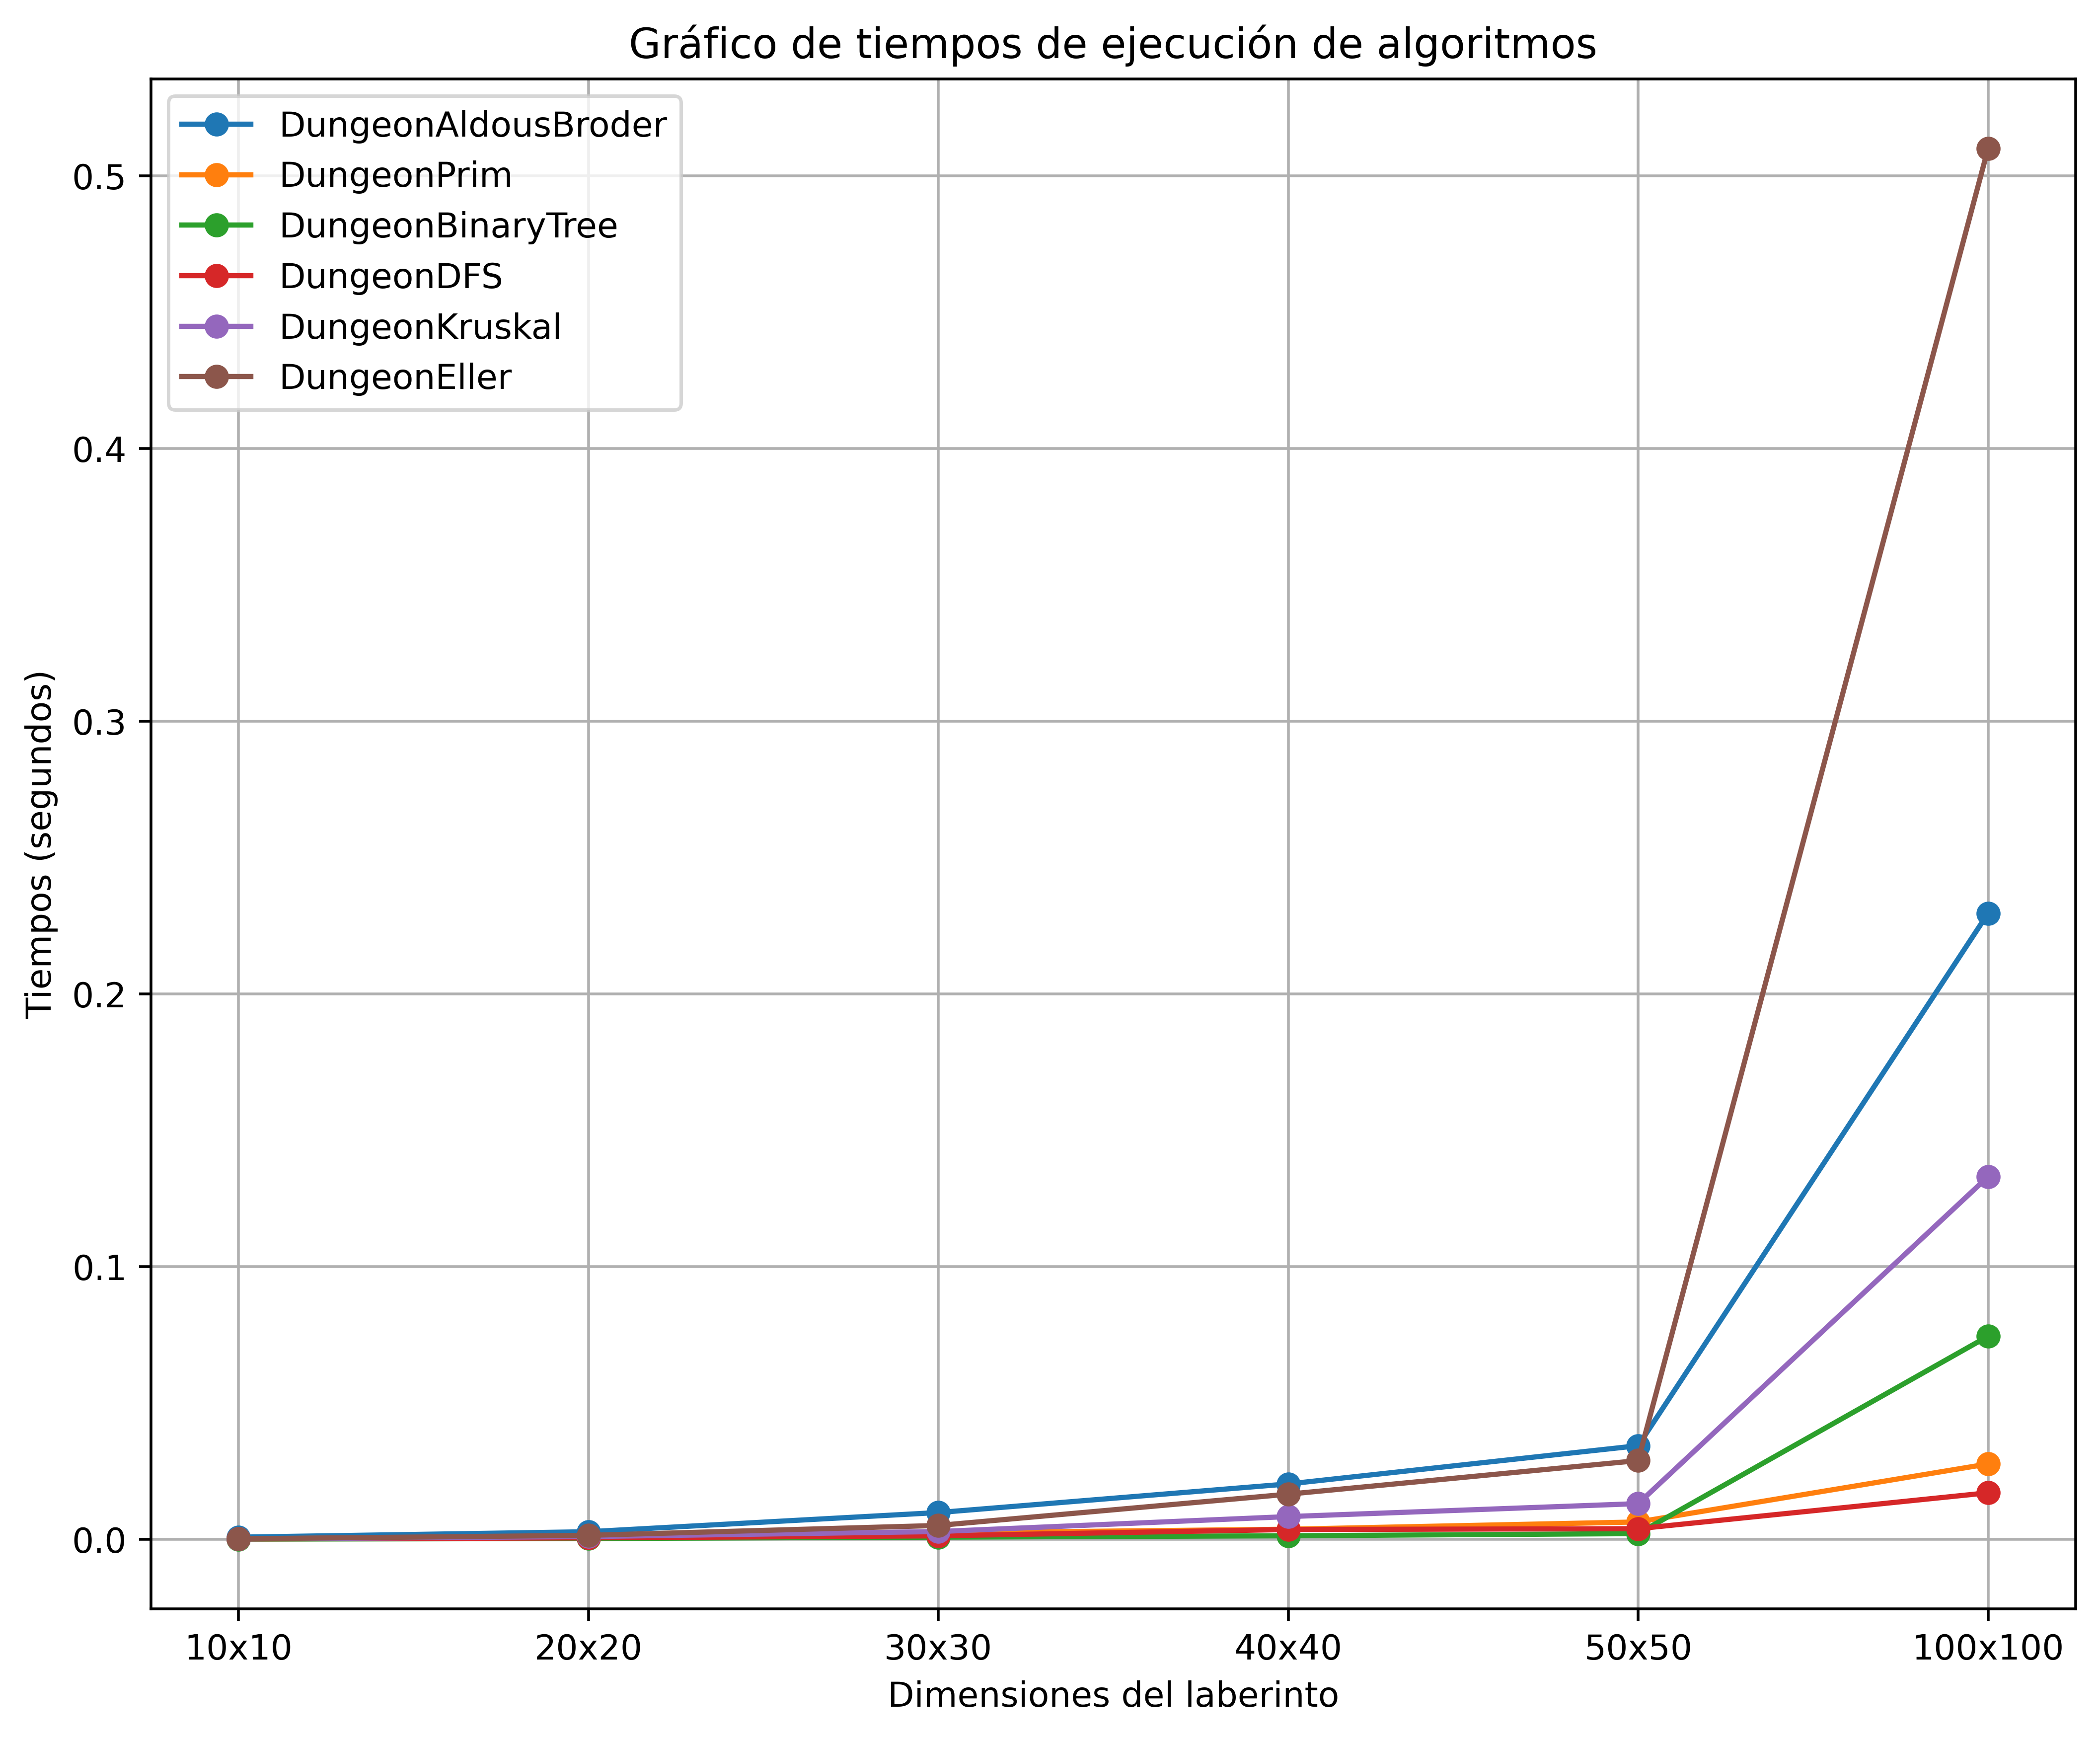
\includegraphics[width=\textwidth]{img/TimeGraph.png}  
    \caption{Gráfico de tiempos de ejecución de algoritmos}  
    \label{fig:TiemposAlgoritmos}
\end{figure}

\begin{figure}
    \centering  
    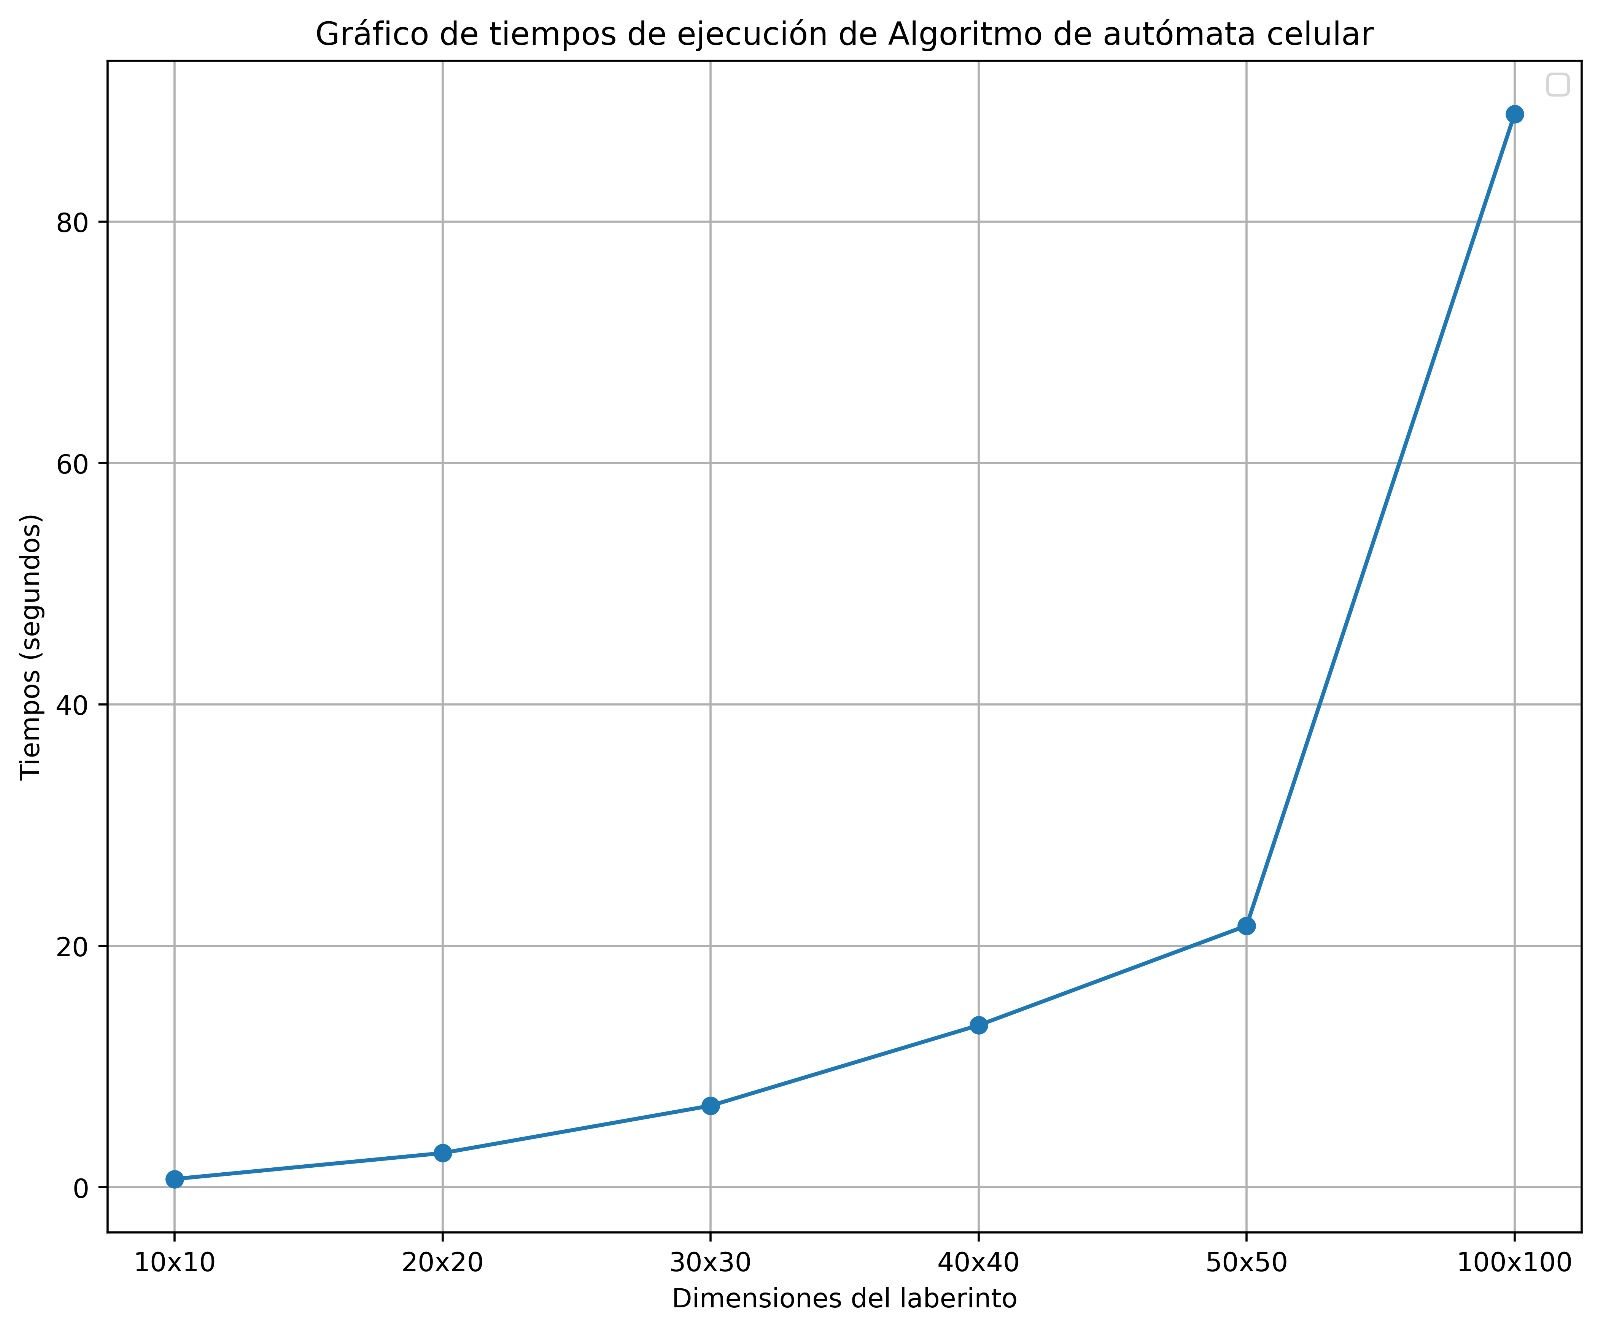
\includegraphics[width=\textwidth]{img/CelularTiempos.jpeg}  
    \caption{Gráfico de tiempos de ejecución de DungeonCelullar.}  
    \label{fig:CelularTiempos}
\end{figure}

\begin{figure}
    \centering  
    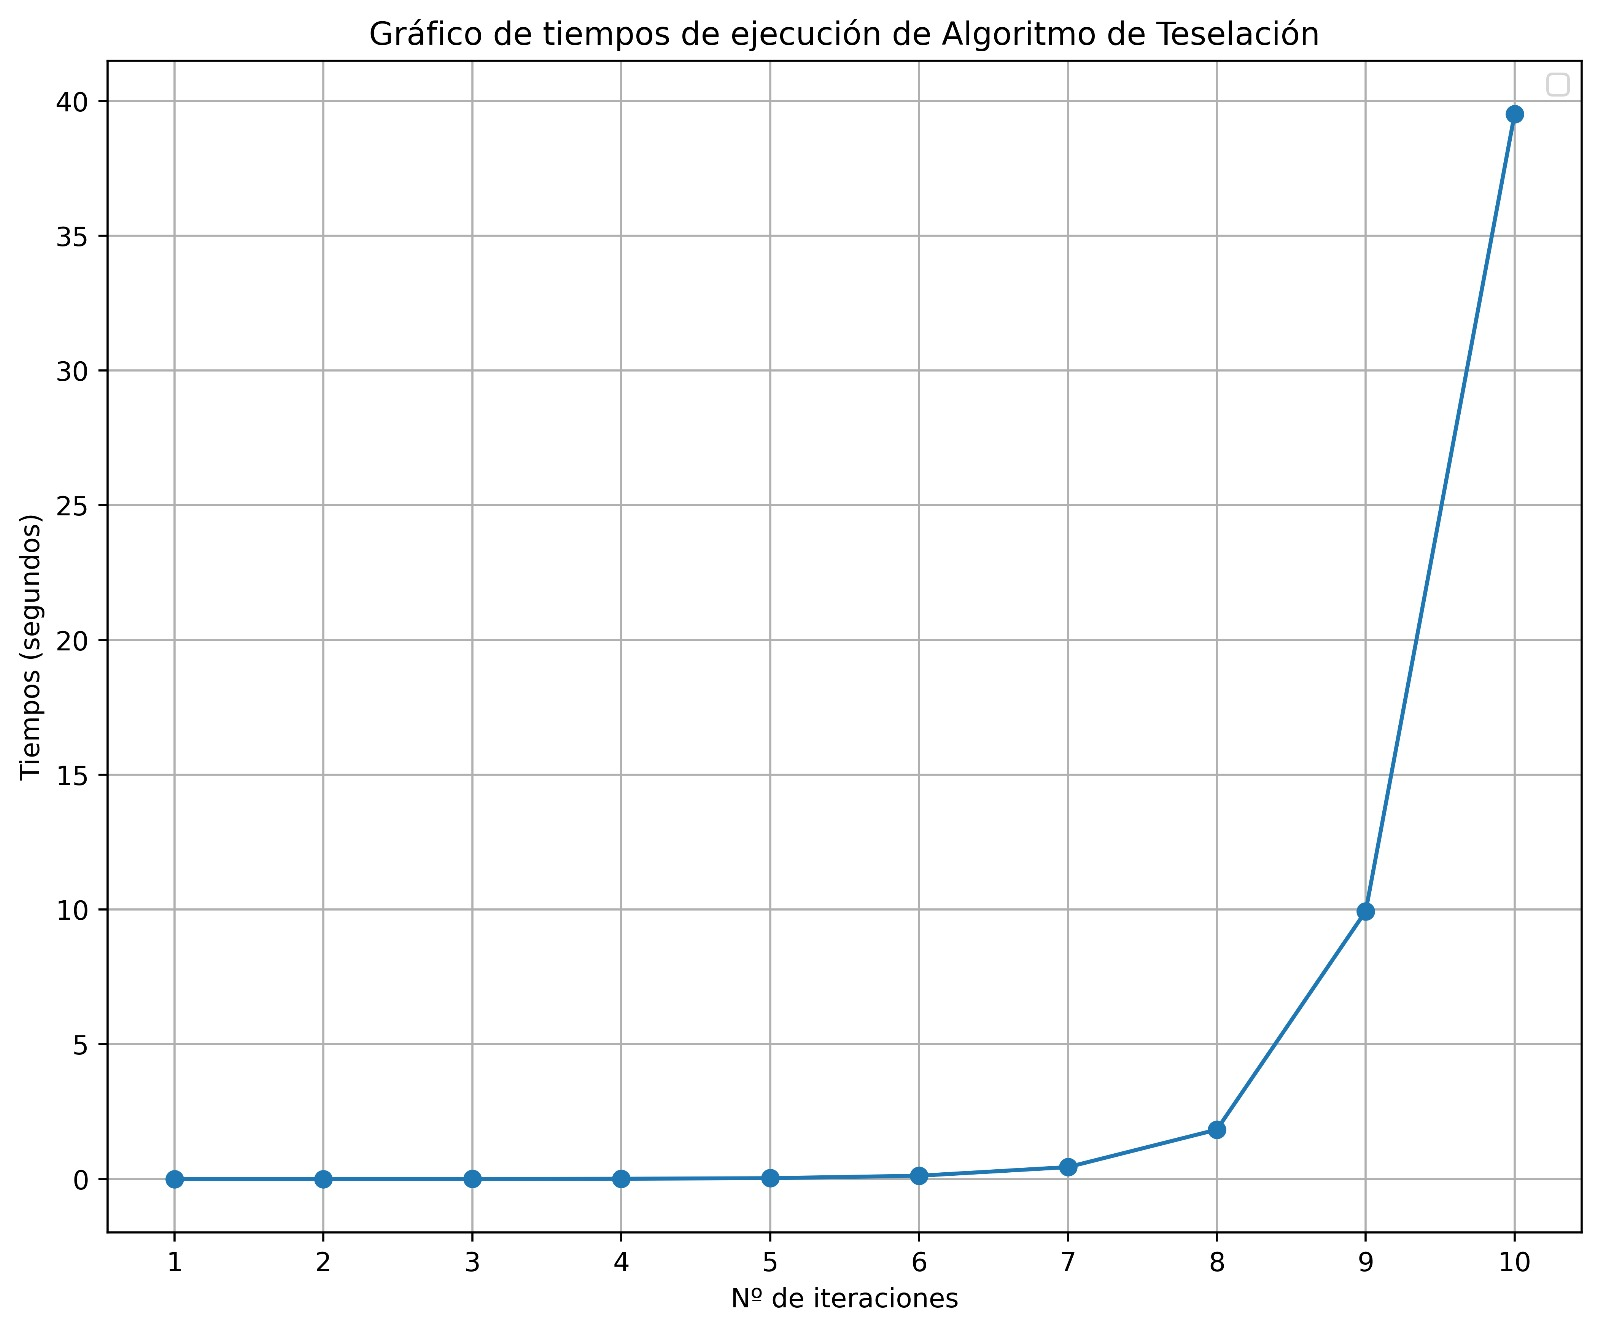
\includegraphics[width=\textwidth]{img/TeselacionTiempos.jpeg}  
    \caption{Gráfico de tiempos de ejecución de DungeonTesselation.}  
    \label{fig:TeselacionTiempos}
\end{figure}

\begin{table}
\centering
\caption{Resultados detallados de tiempos de ejecución de algoritmos (Parte 1)}
\label{tab:resultados_detallados_parte1}
\begin{tabular}{lrrr}
\toprule
          Algoritmo &    10x10 &    20x20 &    30x30 \\
\midrule
DungeonAldousBroder & 0.000524 & 0.005217 & 0.029298 \\
        DungeonPrim & 0.000443 & 0.001009 & 0.002407 \\
  DungeonBinaryTree & 0.000108 & 0.000330 & 0.000840 \\
         DungeonDFS & 0.000161 & 0.000592 & 0.001549 \\
     DungeonKruskal & 0.000200 & 0.001580 & 0.003289 \\
       DungeonEller & 0.000220 & 0.001374 & 0.005380 \\
\bottomrule
\end{tabular}
\end{table}

\begin{table}
\centering
\caption{Resultados detallados de tiempos de ejecución de algoritmos (Parte 2)}
\label{tab:resultados_detallados_parte2}
\begin{tabular}{lrrr}
\toprule
          Algoritmo &    40x40 &    50x50 &  100x100 \\
\midrule
DungeonAldousBroder & 0.027014 & 0.021885 & 0.136055 \\
        DungeonPrim & 0.004057 & 0.006651 & 0.026567 \\
  DungeonBinaryTree & 0.001427 & 0.002176 & 0.007692 \\
         DungeonDFS & 0.002483 & 0.004625 & 0.041779 \\
     DungeonKruskal & 0.006238 & 0.012281 & 0.138475 \\
       DungeonEller & 0.014307 & 0.032310 & 0.483169 \\
\bottomrule
\end{tabular}
\end{table}

\capitulo{4}{Técnicas y herramientas}

En la presente sección se describen las principales técnicas y herramientas con los que se ha trabajado a lo largo del proyecto.

\section{Gestión de proyecto}

\subsection{Overleaf}
La herramienta principal para desarrollar la memoria de este trabajo ha sido Overleaf~\cite{overleaf}. Esta herramienta es un entorno que permite la creación de documentos TeX/LaTeX.
Las principales ventajas de Overleaf son su facilidad de uso y la opción colaborativa, permitiendo añadir a más personas para poder colaborar con el documento.
La herramienta permite el control de versiones de los documentos, permitiendo ver el progreso del desarrollo y haciendo posible volver a versiones anteriores.


\subsection{Scrum}
Scrum~\cite{scrum} es un marco de trabajo ágil que se utiliza para gestionar y realizar proyectos de mayor complejidad.
Se basa en los principios de desarrollo iterativo e incremental, de forma que proporciona un enfoque estructurado y flexible para el desarrollo de productos. Este enfoque es muy eficiente en la gestión de proyectos de software ya que permite al equipo adaptarse rápidamente a los cambios y conseguir una mayor retroalimentación.

Para este proyecto estas iteraciones en las que se basa Scrum (Sprints) han sido de tres a cuatro semanas, puesto que ha sido un proyecto que se ha extendido en el tiempo. Cada final de sprint se realizaba una reunión sobre los progresos y bloqueos que han podido surgir. De esta forma se ha ido iterando a lo largo del tiempo.

\subsection{Jira}
Jira~\cite{jira} es una herramienta de gestión de proyectos y seguimiento de incidencias desarrollada por Atlassian. Es muy popular en la industria del software para llevar una planificación y gestión de proyectos de desarrollo. Es utilizada para metodologías de trabajo como Agile, Scrum y Kanban. 

Para este proyecto ha sido especialmente útil, ya que al usar Scrum, permite seguir el flujo del trabajo y ver en qué punto se encontraba el proyecto con claridad.

\subsection{Git}
Git~\cite{git} es un sistema de control de versiones distribuido, está diseñado para gestionar proyectos con mucho historial y para poder mantener un control de versiones.
Para este proyecto se eligió git ya que es el más popular. Git permite usar la gestión de ramas, es crucial para trabajos en equipo, pero para este proyecto sólo se ha usado la rama principal. La gran ventaja de usar git es que no se necesita conexión constante a internet para trabajar, simplemente con la copia del repositorio en la máquina se pueden subir los cambios cuando sea necesario. 
Git ha sido imprescindible en el desarrollo de este proyecto, facilitando el proceso enormemente.

\subsection{Git Bash}
Git Bash~\cite{gitbash} es una interfaz de línea de comandos que emula un entorno de terminal bash en Windows. Con esta herramienta se pueden usar comandos de Git y Unix para gestionar repositorios de git. 
También tiene soporte para scripts de bash, permitiendo automatizar trabajo desde la terminal como si se tratase de una terminal de Unix. 
Para el desarrollo de este proyecto fue fundamental ya que se utilizó para gestionar el repositorio, y es igual de fácil de usar que una terminal de un sistema Unix.


\section{Lenguajes de programación}
\subsection{Python}
Python~\cite{python} es un lenguaje de programación de alto nivel, destaca por ser simple y legible. Es muy utilizado para el desarrollo de aplicaciones gracias a su compatibilidad con diversidad de frameworks. También cuenta con una gran cantidad de bibliotecas para poder trabajar en diferentes dominios, ya sea para desarrollar los algoritmos de generación procedimental, como para desarrollar el framework.

\subsection{C\#}
C\#~\cite{csharp} es un lenguaje de programación orientado a objetos, desarrollado por Microsoft como parte de su plataforma .NET. Unity utiliza este como el lenguaje principal para scripting, permitiendo así el programar el control de los objetos, el manejo de eventos y la interacción del usuario.
Este lenguaje es conocido por tener una sintaxis clara y gracias a su gran comunidad de usuarios se dispone de mucha documentación, haciendo la curva de aprendizaje mucho más suave.


\section{Bases de datos}

\subsection{MongoDB}
MongoDB~\cite{mongodb} es una base de datos NoSQL orientada a documentos. Este tipo de base de datos hace que sea más fácil almacenar datos de forma flexible puesto que es capaz de manejar grandes volúmenes de datos, además de que permite la escalabilidad de la base de datos.

Uno de los principales motivos por los que se eligió esta base de datos es por su \textbf{modelo de datos flexible}, MongoDB tiene capacidad para manejar datos no estructurados, y la flexibilidad en el esquema hace que sea posible adaptarse a los cambios de requisitos sin tener que modificar la estructura de la base de datos. Además se integra muy bien con Docker, haciendo mucho más fácil el despliegue y la gestión de las bases de datos. Para integrar MongoDB con FastApi se hace uso de dos bibliotecas de Python, Beanie y Pydantic, de los que se hablará en más profundidad en el siguiente apartado.

También, cabe destacar que al  ser muy popular dentro de la comunidad, la documentación es muy completa, esto fue decisivo a la hora de elegir esta base de datos, ya que hace que el aprendizaje y la resolución de errores sea mucho más sencilla.

\section{Bibliotecas}

\subsection{Beanie}
Beanie~\cite{beanie} es una biblioteca para Python diseñada para trabajar con bases de datos MongoDB en un estilo orientado a documentos, es decir, es un \textbf{ODM (Object-Document Mapper)}. Esto significa que va a utilizar clases y objetos en lugar de consultas SQL, facilitando la manipulación de datos de forma que es más coherente con la programación orientada a objetos porque proporciona una interfaz de alto nivel para interactuar con la base de datos. 

Usar un ODM en este proyecto permite que los esquemas de datos sean flexibles, haciendo el almacenamiento mucho más sencillo.

La integración con FastApi de MongoDB fue posible gracias a \textbf{Beanie}, esta biblioteca facilita la integración ya que usa modelos de datos definidos con Pydantic. 

\subsection{Pydantic}
Pytdantic~\cite{pydantic} es una biblioteca para Python que hace más fácil la validación y conversión de datos mediante el uso de anotaciones de tipos.
Pydantic define modelos de datos, en este caso para crear clases modelos, esto permite una validación y conversión de datos a tipos específicos de Python, haciendo que los datos tengan una mejor consistencia y calidad al almacenarse. También se usa Pydantic con FastApi, haciendo que la validación y conversión de datos sea robusta y coherente entre el framework web y la base de datos.

\section{API}

\subsection{FastAPI}
FastAPI~\cite{fastapi} es un framework web de alto rendimiento para construir APIs en Python 3.7+, basado en estándares como OpenApi y JSON Schema. 

FastAPI era la mejor elección para usarlo como framework por diversos motivos. Ofrece un \textbf{rendimiento muy alto}, haciéndolo la mejor elección en una aplicación en la que se necesita una buena capacidad de respuesta.
También, FastApi permite desarrollar de forma más \textbf{rápida y sencilla}, sobre todo por la generación de documentación que ofrece, que permite desarrollar APIs más rápido y con menos errores.
Además, facilita mucho la generación de la documentación según la especificación de OpenAPI.

Por estos motivos es la mejor elección para desarrollar APIs eficientes y escalables, hace mucho más fácil el desarrollo y mantenimiento del back-end de una aplicación.

\subsection{Uvicorn}
Uvicorn~\cite{uvicorn2024} es un servidor ASGI (Asynchronous Server Gateway Interface) ultrarrápido, basado en Python, diseñado para proporcionar un rendimiento óptimo en aplicaciones web asincrónicas. Es el servidor elegido para el desarrollo del back-end de este proyecto porque es muy práctico para proyectos que necesitan una alta capacidad de respuesta y poca latencia, como aplicaciones en tiempo real y APIs.

La principal ventaja de uvicorn es la capacidad para manejar \textbf{múltiples conexiones simultáneas} eficientemente, esto es gracias a su arquitectura basada en el bucle de eventos de asyncio. Lo hace excelente para aplicaciones que necesitan mucha concurrencia, como pueden ser los videojuegos. 

En este proyecto, Uvicorn se utiliza como el servidor de back-end para desplegar la API desarrollada, garantizando un rendimiento robusto y una fácil escalabilidad.

\section{Gestión y despliegue de contenedores}

\subsection{Docker}
Docker~\cite{docker} es una plataforma que permite empaquetar aplicaciones y sus dependencias en contenedores. De esta forma se asegura de que estas se ejecuten de manera consistente en cualquier entorno.

Docker en el caso de este proyecto, \textbf{aísla las dependencias}. Esto significa que empaqueta todas las dependencias de FastApi en un contenedor, así asegura el funcionamiento de manera consistente en diferentes entornos sin problemas de compatibilidad. En cada uno de los contenedores se va a ejecutar una instancia de la aplicación aislada del sistema operativo anfitrión y de otros contenedores. Esto también lo hace más seguro y estable a los cambios, asegurando que las aplicaciones se ejecuten de forma idéntica en cualquier entorno, sea una máquina local, la nube o servidores de producción.

Docker va a permitir que se cree una imagen del contenido que va a contener todo lo necesario para ejecutar la aplicación, haciendo que el \textbf{despliegue sea consistente} en cualquier servidor o plataforma de nube.

\subsection{DevContainers}
Para poder hacer portable la aplicación se hace uso de un Devcontainer. DevContainer~\cite{devcontainers} es un paradigma de uso de contenedores, que gestiona entornos de forma aislada y ligera, permitiendo a un desarrollador trabajar dentro de una versión del entorno, haciendo que esté dentro de un contenedor. 

Un DevContainer puede dar un \textbf{entorno preconfigurado} dentro del IDE. Esto hace que se pueda ahorrar mucho tiempo preparando el proyecto y haciendo que el entorno esté listo cada vez que se arranque el contenedor. Así garantiza que el trabajo se hará en un ambiente consistente y replicable, independientemente de la configuración que se tenga en la máquina local, haciendo que se eliminen los problemas de configuración que pueden surgir en distintos entornos.
Los entornos se definen con archivos de configuración sencillos, haciendo más fácil la creación y gestión de los entornos, incluyendo especificaciones sobre el sistema operativo, herramientas y configuraciones específicas del proyecto. 

Gracias a estas características hace que sea una herramienta muy útil e interesante de utilizar para el desarrollo del proyecto.

\section{Motor de videojuegos}

\subsection{Unity}
Unity~\cite{unity} es un motor de desarrollo de videojuegos, es de los más populares dentro de la industria de videojuegos. Se pueden desarrollar videojuegos 2D, 3D, realidad aumentada y realidad virtual. 

Es un motor muy completo que permite desarrollar y desplegar el juego en varias plataformas como PC, web, realidad virtual y para móvil. 
También tiene muchas \textbf{herramientas de desarrollo integradas}, para preparar las escenas, un sistema de físicas y herramientas de animación. Esto hace mucho más fácil la creación de contenido en tiempo real.


\section{IDEs}
\subsection{Visual Studio Code}
Visual studio code~\cite{vscode} es el IDE elegido para desarrollar el <<Back-end>> de la aplicación. Este entorno de programación es muy versátil y permite trabajar con un gran número de lenguajes de programación, siendo de los más ligeros. 

Para poder trabajar con Docker, se dispone de extensiones que permiten construir, administrar y desplegar contenedores directamente desde el editor. Esto incluye la \textbf{creación y gestión de imágenes Docker}, así como la configuración y ejecución de contenedores y servicios Docker Compose.

Además, VSCode tiene una \textbf{terminal integrada}, esto junto a la posibilidad de tener entornos de desarrollo configurados con Docker, hacen de ese IDE una excelente opción para preparar DevContainers. 


\subsection{Visual Studio}
Visual Studio~\cite{visualstudio} es el IDE usado para desarrollar el código de los scripts del videojuego. Este es muy utilizado para la programación en C\#, el lenguaje principal para la programación en Unity.  

Visual Studio se integra muy bien con Unity, como por ejemplo \textbf{IntelliSense}, que ofrece autocompletado de código para el motor, agilizando el desarrollo y con menos errores. También dispone de \textbf{Visual Studio Tools for Unity(VSTU)} que mejora la productividad al integrar perfectamente las características de Visual Studio con el flujo de trabajo de Unity. Pero lo más importante es que permite depurar proyectos de Unity directamente desde Visual Studio, haciendo más facil identificar y corregir errores.

\section{Otros}
\subsection{Jupyter notebook}
Jupyter Notebook~\cite{jupyter} es una aplicación web de código abierto que permite crear documentos que contienen código ejecutable, ecuaciones, visualizaciones y texto narrativo. Es muy popular ya que se utiliza para la ciencia de datos, investigación y enseñanza, porque permite explorar datos, desarrollo de modelos y tener una documentación interactiva.

Para este proyecto se ha utilizado para poder desarrollar más dinámicamente cada uno de los algoritmos que generan laberintos. Hace que desarrollar y probar sea más rápido, no hay necesidad de arrancar el servidor y Unity para poder ver el resultado, ya que se puede ejecutar y dibujar directamente en el Notebook. 






\capitulo{5}{Aspectos relevantes del desarrollo del proyecto}

El planteamiento de este proyecto ha ido variando durante su desarrollo. Al ser un proyecto de investigación y aprendizaje, el objetivo de este también ha ido evolucionando.
El primer paso del desarrollo del proyecto consistió en hacer una investigación y pruebas de concepto. Se hizo una investigación de qué herramientas podrían ser mejores para el desarrollo de este proyecto.

\section{Java}
La primera prueba de concepto consistió en la elaboración del juego sin motor gráfico, haciéndolo desde cero con el IDE eclipse usando java. El objetivo de la prueba de concepto era conseguir elaborar una pequeña pantalla que imprimiese un laberinto con el algoritmo más sencillo posible. 

El primer paso fue ver cuál podría ser la forma más sencilla de implementar, y se encontró el laberinto de Wilson, aunque no es la forma más eficiente de generar laberintos de mayor tamaño.

Tras esto comenzó el desarrollo de la prueba de concepto, pero no había demasiada documentación online y era muy costoso de realizar por lo que no se terminó la prueba y se descartó.

\section{C\# y .NET}
La segunda prueba de concepto fue desarrollada en C\#, este lenguaje no era la primera opción ya que se carecía de experiencia con él, pero resultó ser muy parecido a java por lo que la curva de aprendizaje fue más suave. Desarrollarlo en .NET tiene como gran desventaja que a la hora de escalarlo y hacer mazmorras, es muy limitante. Hace que resulte muy costoso dibujar el mapa, por lo que esta opción fue también descartada antes de terminar la prueba de concepto.

\section{Unity - Primera fase}
La tercera prueba de concepto se realizó de una forma mucho más cómoda que las dos anteriores. Al ser un motor de videojuegos, tiene una comunidad mucho mayor, lo que ayudó en el desarrollo de esta misma. La prueba de concepto consigue lograr el objetivo y con muy poco código tener el generador de laberintos funcionando.

Esta primera fase del proyecto tenía como objetivo que dibujase en 2D un laberinto y que este fuese jugable.
La parte principal, consiste en una matriz en la que vamos a ir alterando con un algoritmo si hay o no una pared, y esto lo iríamos dibujando por toda la matriz. 

\begin{algorithm}
\caption{GenerarLaberinto}
\begin{algorithmic}
\Procedure{GenerarLaberinto}{tamañoX, tamañoY}
    \State laberinto = nuevo arreglo bidimensional de enteros con tamaño (tamañoX, tamañoY)
    \State entero maxX = obtenerLímiteSuperior(laberinto, 0)
    \State entero maxY = obtenerLímiteSuperior(laberinto, 1)
    
    \For{entero i desde 0 hasta tamañoX}
        \For{entero j desde 0 hasta tamañoY}
            \If{i == 0 o j == 0 o i == maxX o j == maxY}
                \State laberinto[i][j] = 1
            \Else
                \If{i es par y j es par}
                    \If{valorAleatorio() > umbralColocación}
                        \State laberinto[i][j] = 1
                        \State entero a, b
                        \If{valorAleatorio() < 0.5}
                            \State a = 0
                        \Else
                            \If{valorAleatorio() < 0.5}
                                \State a = -1
                            \Else
                                \State a = 1
                            \EndIf
                        \EndIf
                        \If{a != 0}
                            \State b = 0
                        \ElsIf{valorAleatorio() < 0.5}
                            \State b = -1
                        \Else
                            \State b = 1
                        \EndIf
                        \State laberinto[i + a][j + b] = 1
                    \EndIf
                \EndIf
            \EndIf
        \EndFor
    \EndFor
\EndProcedure
\end{algorithmic}
\end{algorithm}

En el pseudocódigo de \emph{Algorithm 1} se puede observar que tiene ciertas características y estructuras algorítmicas que son similares a las que se utilizan en el <<Laberinto de Wilson>>, un algoritmo de generación de laberintos que funciona eligiendo un punto de inicio aleatorio y extiende caminos desde él hasta que se conecta con un camino existente. No es idéntico, pero comparte la idea de crear caminos aleatorios dentro de un área determinada.

El laberinto resultante tenía el aspecto de la figura \ref{fig:PrimerLaberinto}.
\begin{figure}[hb]  
    \centering  
    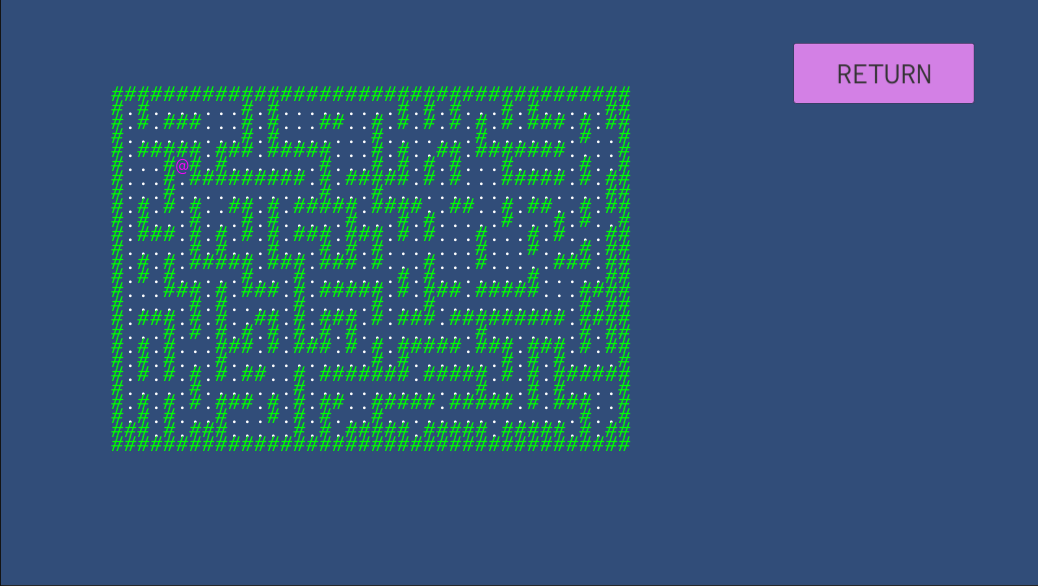
\includegraphics[width=\textwidth]{img/PrimerLaberinto.png}  
    \caption{Primer laberinto generado en Unity.}  
    \label{fig:PrimerLaberinto}
\end{figure}

Cuando se renderiza o <<dibuja>> el mapa con el jugador (representado por el icono @), cada vez que este icono se movía, internamente en Unity se obligaba a dibujar el mapa al completo. Esto es muy ineficiente, para solucionar este problema, en la siguiente iteración, ya se comienza a hacer uso del objeto que Unity proporciona, \texttt{GameObject}.

Un \texttt{gameObjects}~\cite{UnityGameObject} es la unidad básica de organización y representación en una escena, es similar a un objeto en java. En este caso convertir al jugador en un \texttt{gameObjects} nos quitará la necesidad de ir dibujando constantemente el mapa, y entran en juego las animaciones en tiempo real que realiza el motor.

Tras comenzar a refactorizar el proyecto de Unity, se llegó a la conclusión de que era mucho más eficiente empezar un proyecto desde cero, por ello se creó la carpeta <<SegundaFase>>, en esta se realizaría el proyecto de una forma más organizada. Habría consumido mucho más tiempo intentar refactorizar todo el proyecto anterior.


\section{Unity - Segunda fase}
En esta segunda fase, el proyecto a desarrollar cambia por completo. Ahora el proyecto va a imitar la arquitectura cliente - servidor que se emplea en la industria, el servidor va a enviar al cliente, en este caso Unity, lo que tiene que dibujar.

\subsection{Preparación del back-end}
Las primeras semanas fueron para investigar cómo construir este servidor y cual sería la forma más sencilla de hacerlo. 
\subsubsection{Construcción de la API}
Para \textbf{construir la API}, la elección fue FastAPI, ya que al ser tan popular, hay mucha documentación, haciendo la curva de aprendizaje más suave. Una de las grandes ventajas de FastAPI es su documentación automática, desde la que se puede testear la API directamente, sin necesidad de desarrollar interfaz gráfica. Esto hizo los primeros pasos muy dinámicos, ya que el esfuerzo se podía centrar en desarrollar el servidor y los algoritmos.

\subsubsection{Preparación de los algoritmos}
Los \textbf{algoritmos} se desarrollaron en Python, y el servidor se va a encargar de generarlos, almacenarlos y enviar el resultado en forma de JSON al cliente. Este luego se encargará de leer y dibujar en el motor para que sean jugables. 

Muchos de los algoritmos primero fueron desarrollados en un Notebook de Jupyter en paralelo, así se facilita el desarrollo sin necesidad de tener que ir probando con Unity para ver cómo se dibujan. Cuando ya se tenía el algoritmo funcional, se necesitó ir adaptando ya que al principio no se estaba teniendo en cuenta la semilla para la generación de estos laberintos.

\subsubsection{Preparación de la base de datos}

Para poder \textbf{almacenar información} en la base de datos al principio se pensó que la mejor opción era SQLite, y se comenzó a desarrollar. 
SQLite, que es SQL, tiene la desventaja de que utiliza un modelo relacional con tablas y esquemas rígidos, y esto quita una flexibilidad muy necesaria cuando se decidió cambiar el modelo de datos. 

Un cambio importante en el almacenamiento de los laberintos surgió cuando se pensó en que era más óptimo almacenar los laberintos al completo, junto con su \textbf{semilla}. Esto se debe a que la generación procedimental es determinista, es decir, que con las mismas entradas se produce la misma salida, por ello es tan eficiente y útil almacenar la semilla.

Para hacer esto se cambió a una base de datos \textbf{NoSQL}, está orientada a documentos que almacena datos en formato BSON. Esto ofrece mucha más flexibilidad, haciendo que los datos no estén semi-estructurados, así si los datos cambian con el tiempo se puede adaptar. Este cambio nace por la inmediatez que ofrece al acceder a los laberintos y que desaparece la necesidad de establecer relaciones entre entidades. MongoDB ofrece replicación y tolerancia a fallos haciendo que los datos estén disponibles incluso en caso de problemas de hardware o red.


\subsection{Preparación del juego}
Para poder usar Unity como cliente, una parte clave ha sido \textbf{UnityWebRequest}, esta clase permite realizar llamadas HTTP, pudiendo así conseguir llamar al servidor con el algoritmo que seleccionado y para que devuelva el laberinto generado. 
Cuando Unity recibe el .JSON, lo transforma y con la matriz resultante que ha enviado el servidor, lo dibuja.

En Unity para este proyecto se han creado varios scripts, tanto para el control del <<Menu>> y de las pantallas como para poder dibujar en el motor y navegar el mapa. 

Gracias al sistema de físicas que tiene Unity por defecto, ha sido mucho más sencillo desarrollar el juego, utilizando mallas (Mesh~\cite{unitymesh}). Una malla consiste en una gran cantidad de triángulos y vértices que definen la forma de un objeto tridimensional, almacenados en un array, esta malla se podría poner rodeando al objeto 3D deseado y hacer que se comporte como material físico. Esto es lo que va a rodear a los cubos que van a interactuar como paredes para el jugador, de lo contrario el jugador podría atravesar el laberinto. Esto va a ir programado en un script que luego se va a cargar en el <<GameManager>>, el objeto que va estar encargado de cargar los scripts asociados.

Para que la cámara no se quede estancada y pueda seguir al jugador, hace falta un script que vaya a tiempo real con el jugador. Para ello hizo falta encontrar la rotación adecuada. Fue una tarea de prueba y error, hasta que se decidió no rotar la cámara porque se perdía visibilidad de la bola.

El evento para que cargue la escena hace también la llamada al servidor, entre escenas no se almacena la información, por lo que para poder guardar lo que el usuario haya seleccionado y se pueda enviar en la llamada, fue clave el uso de <<PlayerPreferences>>~\cite{unityplayerprefs}, es una clase de Unity que en la que se puede cargar la información y aunque se cambie de escena esta información no se pierde, por lo que se puede volver a cargar en las escenas que se necesiten.


\capitulo{6}{Trabajos relacionados}

En este apartado se van a observar distintas herramientas que como producto final generan mazmorras y con qué finalidad se utilizan.
Existen gran variedad de herramientas/juegos, tanto de pago como gratuitos en plataformas como itchio~\cite{itchio}, pero los siguientes engloban muy bien qué hay disponible.

\section{DunGen}
DunGen~\cite{DunGen} es una API web en la que se pueden generar mazmorras de alta resolución en dos dimensiones. Las mazmorras generadas se pueden descargar en formato .jpg de forma gratuita.

Este generador, ofrece incluir que sea multi-nivel, es decir, que tiene más de una planta además de que ofrece 8 temáticas para poder elegir, cambiando el aspecto de una mazmorra normal a una con temática de hielo. 
En esta herramienta, también se puede introducir si se desea la semilla al igual que en este proyecto.

Algo que no incluye es que poder introducir las dimensiones deseadas, en este caso da unas medidas por defecto y genera el resultado.
El resultado de una mazmorra generada tiene el aspecto de la figura 6.1.
\begin{figure}[ht!]  
    \centering  
    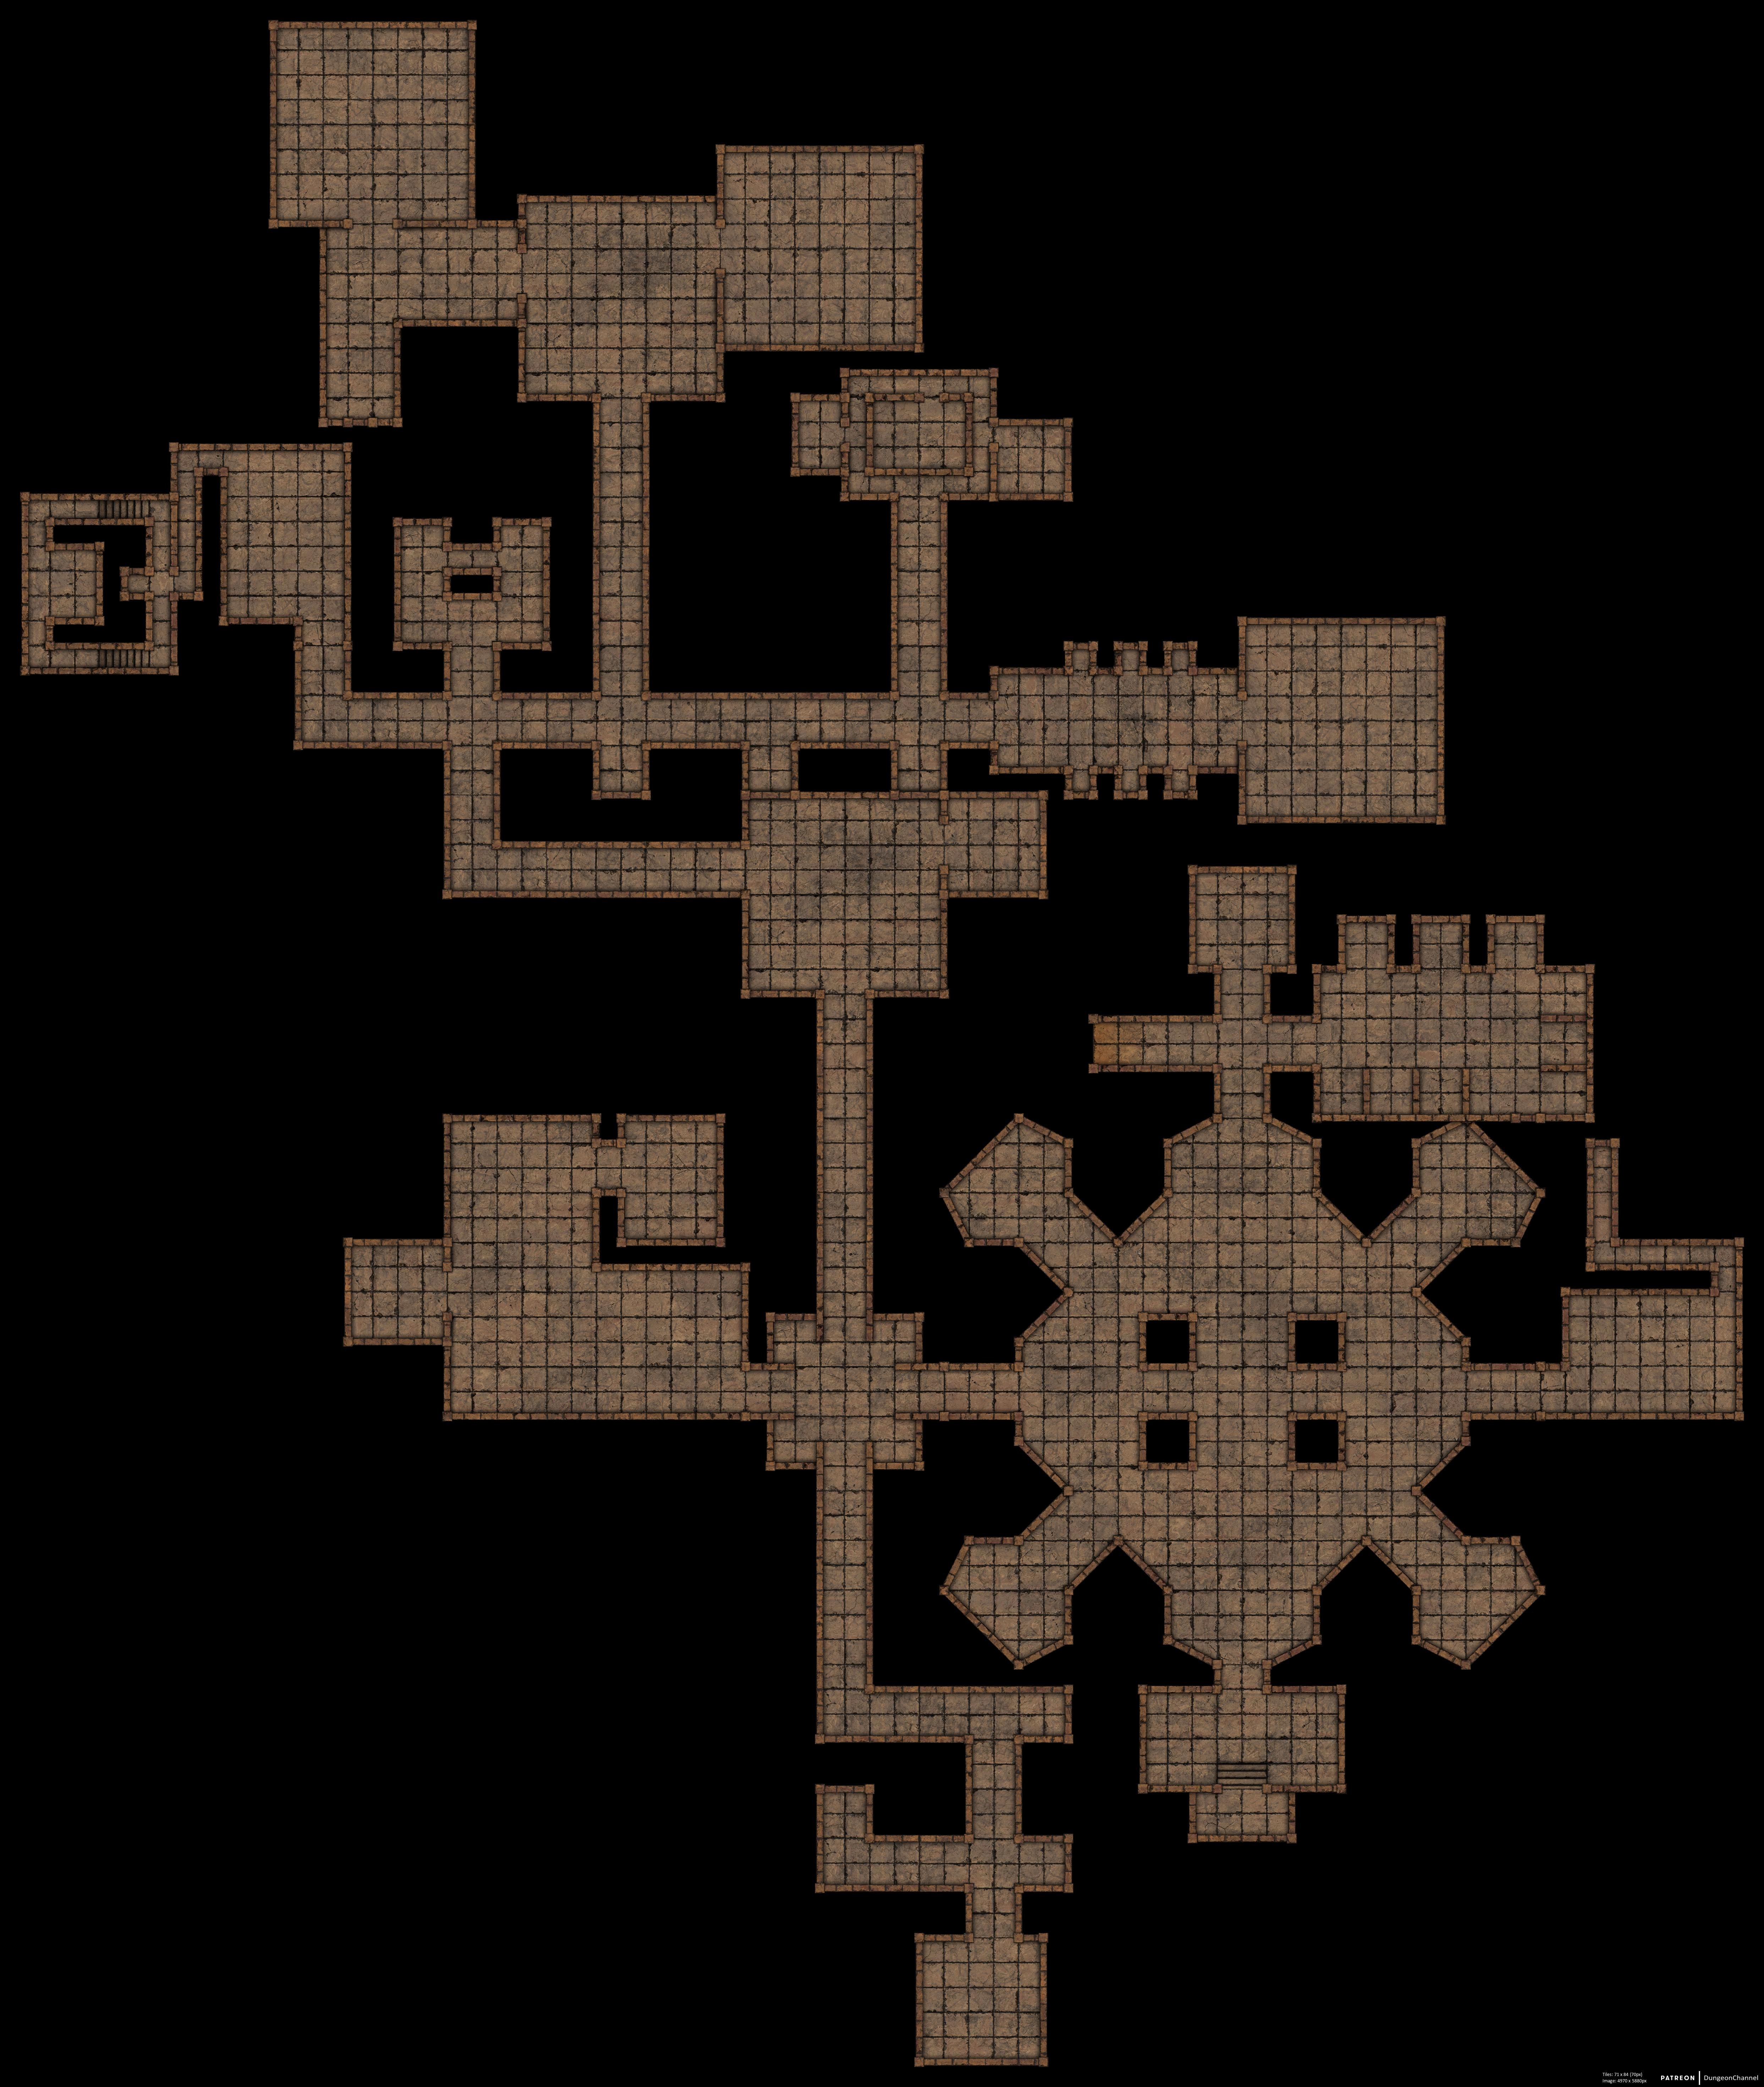
\includegraphics[width=\textwidth]{img/DunGenMediumExample.jpg}  
    \caption{Mazmorra generada con DunGen Dungeon Generator. Extraído de \url{https://dungen.app/dungen/}  }
    \label{fig:MazmorraDunGen}
\end{figure}

\section{Donjon}
Donjon~\cite{Donjon} es una API web que genera contenido para juegos de rol. Tiene un apartado para generar mazmorras, pero también genera gran cantidad de cosas como las puntuaciones de los enemigos o nombres de fantasía. Todo el contenido se puede descargar en varios formatos, haciendo de esta herramienta una muy versátil.
Este es un gran ejemplo de aplicación de generación de contenido fuera del ámbito de los videojuegos, funciona como herramienta de apoyo para crear un juego de mesa de rol propio.

La generación de mazmorras funciona de una forma similar a DunGen, mencionado anteriormente, pero a diferencia del anterior, este ofrece mucha más personalización, como por ejemplo, deja elegir si va a tener escaleras o si tiene puertas. Pero al igual que en el caso de DunGen, los parámetros ya están definidos, incluyendo el tamaño, es decir, no deja al usuario introducir manualmente el tamaño deseado.
Un ejemplo de resultado generado en Donjon tendría el aspecto de la figura \ref{fig:LabyrinthDonjon}.
\begin{figure}[h]  
    \centering  
    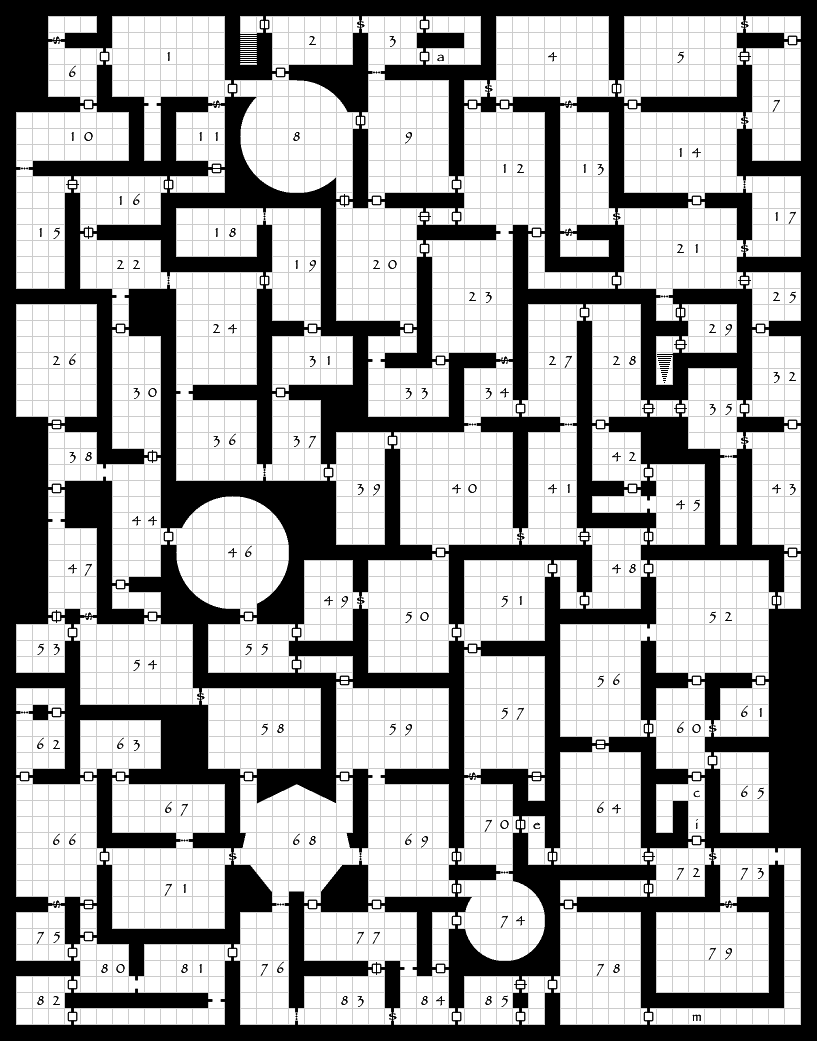
\includegraphics[width=\textwidth]{img/LabyrinthDonjon.png}  
    \caption{Mazmorra generada con Donjon.  Extraído de \url{https://donjon.bin.sh/d20/dungeon/}}  
    \label{fig:LabyrinthDonjon}
\end{figure}



\section{Endless RPG}

Endless RPG ~\cite{Endlessrpg}, es un juego de pago que genera mapas para Dragones y Mazmorras con enemigos y elementos clave para poder desarrollar la partida. El juego permite a los jugadores explorar la mazmorra y enfrentarse a los enemigos de la misma forma que se hace en una partida de rol, es decir, con un organizador de la partida que va gestionando los turnos y cómo los jugadores interactúan con el entorno. 

En este caso ya no es una herramienta para sólo generar mapas (o contenido), si no para poder jugar directamente, es muy completa y permite a los usuarios personalizar los mapas posicionando elementos para que los descubran los jugadores, como cofres y llaves para poder avanzar por las mazmorras.


\section{Maze Generator}
Más similar al resultado de este proyecto, Maze Generator~\cite{mazegenerator} es una herramienta que genera laberintos en 2D. Permite generar mazmorras de forma gratuita, se le pueden proporcionar datos como su ancho alto, desde dónde se comienza a recorrer el laberinto y el estilo de este. También permite exportar el laberinto generado a pdf o como imagen.
En este caso sí se pueden introducir las dimensiones deseadas pero no se tiene en cuenta la semilla. Tendría el aspecto como el de la figura \ref{fig:MazeGenerator}.
\begin{figure}[h]  
    \centering  
    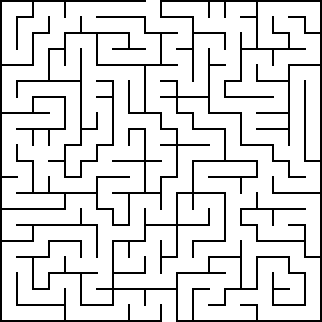
\includegraphics[width=\textwidth]{img/MazeGeneratorExample.png}  
    \caption{Laberinto generado con Maze Generator.}  
    \label{fig:MazeGenerator}
\end{figure}



\capitulo{7}{Conclusiones y Líneas de trabajo futuras}


\section{Conclusiones}
En este proyecto se ha conseguido realizar un juego en el que se generan laberintos de forma procedimental y que son navegables. 
Como se ha mencionado en el apartado de aspectos relevantes del desarrollo, en este proyecto han surgido bastantes dificultades y se ha experimentado, haciendo que cambien los objetivos del proyecto. Se ha ido probando y cambiando hasta encontrar la herramienta más indicada para desarrollar el juego. 

También es un proyecto que se ha alargado bastante en el tiempo, por lo que el conocimiento adquirido en el entorno laboral ha influido en las decisiones sobre qué herramientas y técnicas son más adecuadas.

\subsection{Servidor}
En un principio para este proyecto no se pensó en almacenar los laberintos en una base de datos. Pero tras comenzar el proyecto, fue una idea muy positiva.

Usar FastAPI, gracias a toda la documentación que hay disponible, tuvo una curva de aprendizaje más suave, pero ya que se carecía de experiencia, preparar el servidor llevó una gran cantidad de tiempo y surgieron muchos bloqueos. 

Encontrar qué tipo de base de datos tampoco fue tarea fácil, ya que al principio no se tuvo en cuenta cuál era mejor para almacenar los laberintos. Pero como se ha mencionado en aspectos relevantes del desarrollo, al ir avanzando, se llegó a la conclusión de que MongoDB era la mejor opción. De nuevo, gracias a la cantidad de documentación disponible se suaviza la curva de aprendizaje.
\subsection{Unity}

Antes de empezar a utilizarlo se barajaron muchas otras alternativas, pero fue la mejor entre todas las opciones. Cabe mencionar que aprender a usar Unity, cuando no se ha trabajado antes con un motor de videojuegos, consume mucho tiempo, requiere aprender muchos conceptos y desenvolverse al principio es costoso.
Si no se ha trabajado antes con Unity, es algo muy importante a tener en cuenta, ya que puede que exista otra alternativa en caso de querer realizar una herramienta.

Pero para trabajar en un videojuego, es el mejor motor para comenzar. Ofrece todo lo que se necesita, como elementos para la UI, una exportación del juego con ejecutable, objetos predefinidos, etc. Ahorra tiempo de desarrollo ya que se puede hacer uso de todo lo que ofrece el motor.

Uno de los elementos que ofrece es UnityWebRequest, de no tenerla habría que preparar una clase desde cero para conectar el juego con el servidor. Gracias al manejo de solicitudes, y la compatibilidad con JSON hacen de esta clase que sea extremadamente útil, ahorrando una gran cantidad de tiempo y simplificando la integración con APIs y servicios web. 
Cuando se eligió el motor no se tenía en cuenta este factor, pero cuando se eligió conectar el juego con un servidor, hizo el trabajo mucho más sencillo.

Unity también ofrece objetos predefinidos, haciendo que no sea necesario diseñar objetos en 3D. Permite al desarrollador construir y estructurar juegos mucho más rápido sin necesitar conocimientos de modelado 3D. Lo mismo ocurre para construir la UI, ofrece botones y objetos sencillos para poder construir una UI de forma sencilla y rápida sin necesidad de preparar los botones manualmente.

Si se quieren modificar cosas a bajo nivel es más limitante ya que no deja modificar o reescribir los elementos que ofrece, pero para conseguir desarrollar un videojuego ofrece una implementación de todos los elementos que se necesitan, haciendo de esta herramienta una muy completa. 


\section{Líneas de trabajo futuras}

%Explorar y optimizar los algoritmos

\subsection{Introducción de seguridad en las comunicaciones}
Una línea de trabajo que no se ha podido explorar es introducir usuarios. Cada usuario podría almacenar sus laberintos y poder volverlos a jugar. Es un cambio que exigiría introducir un cifrado de mensaje, ya que en el estado que se encuentra el proyecto, la comunicación está visible y se podría obtener la información que maneja. 

Al no trabajar con usuarios, no hay información que sea comprometida, pero sigue siendo un fallo de seguridad grave.
Debido a que no se puede establecer una relación entre usuario y peticiones realizadas al servidor, se deja abierta la puerta a un uso indebido del servicio. Esto puede hacer que usuarios malintencionados puedan tirar el servicio realizando peticiones de forma masiva.
No se ha podido trabajar en la seguridad por falta de tiempo pero sería algo a mejorar en un futuro de este proyecto. Introducir usuarios también traería la necesidad de implementar un protocolo de autenticación.

\subsection{Transformar laberintos a mazmorras}
En el estado en el que se encuentra, ahora mismo no son mazmorras ya que carece de la generación de habitaciones. Es un cambio que exigiría adaptar todos los algoritmos, por lo que no se ha podido explorar. 
Pero convertiría esta herramienta en un generador de mazmorras explorables.
En esta línea, también sería muy positivo incluir elementos con los que el jugador pueda interactuar, como mapas, llaves y puertas para acceder a nuevas mazmorras. 

\subsection{Algoritmos de resolución}
Un cambio positivo para una línea futura de trabajo sería la implementación de un sistema de ayuda para el jugador que resuelva el laberinto, de forma que aparezca una guía que resuelva el laberinto. En caso de que se pierda el jugador, podría disponer de un botón que le indique el camino de salida del laberinto o mazmorra.

\subsection{Despliegue en un servidor externo}
Para que sea accesible a todos los clientes del servidor, se podría plantear hacerlo público con acceso mediante la API-Key para que se pueda hacer uso de los laberintos generados por el servicio. El desplegarlo en un servidor externo abre la puerta a poder distribuir el juego y que este funcione sin necesidad de tener desplegado el servidor localmente.


\bibliographystyle{plain}
\bibliography{bibliografia}

\end{document}
